% !TeX program = xelatex
\documentclass[UTF8,a4paper,zihao=-4]{ctexart}

\usepackage{geometry}
\geometry{left=2.25cm,right=2.25cm,top=2.35cm,bottom=2.35cm}
\usepackage{graphicx}
\usepackage{float}
\usepackage{booktabs}
\usepackage{longtable}
\usepackage{array}
\usepackage{makecell}
\usepackage{caption}
\usepackage{fancyhdr}
\usepackage{xcolor}
\usepackage{amsmath,amssymb}
\usepackage{enumitem}
\usepackage[hidelinks]{hyperref}
\usepackage{tabularx}
\usepackage{listings}
\usepackage{fontspec}
\usepackage{fvextra}
\setmonofont{DejaVu Sans Mono}
\usepackage[backend=bibtex,style=gb7714-2015]{biblatex}
% \addbibresource{ref.bib}

\captionsetup{font=small,labelfont=bf,justification=centering}
\setlist{nosep,leftmargin=2em}
\setlength{\parindent}{2em}
\setlength{\parskip}{0.15em}
\renewcommand{\arraystretch}{1.08}
\setlength{\tabcolsep}{3pt}
\setlength{\LTpre}{4pt}
\setlength{\LTpost}{6pt}
\setlength{\headheight}{21pt}
\pagestyle{fancy}
\fancyhf{}
\fancyhead[L]{\raisebox{-0.1\height}{
\includegraphics[height=0.85cm]{figures/cicc_logo_small.jpg}}}
\fancyhead[C]{竞业达杯初赛CPU测评报告}
\fancyfoot[C]{\thepage}

\newcommand{\code}[1]{\texttt{\detokenize{#1}}}
\newcommand{\sigs}[1]{\texttt{#1}}
\newcolumntype{L}[1]{>{\raggedright\arraybackslash}p{#1}}
\newcolumntype{C}[1]{>{\centering\arraybackslash}p{#1}}
\newenvironment{tighttable}{%
  \begingroup\zihao{6}\setlength{\tabcolsep}{2pt}\renewcommand{\arraystretch}{1.05}%
}{\endgroup}
\newenvironment{normaltable}{%
  \begingroup\zihao{6}\setlength{\tabcolsep}{2pt}\renewcommand{\arraystretch}{1.05}%
}{\endgroup}

\sloppy

\begin{document}

\begin{titlepage}
  \thispagestyle{empty}
  \centering
  \vspace*{0.6cm}
  {\zihao{1}\bfseries 第十届\par}
  \vspace{0.35cm}
  {\zihao{1}\bfseries 全国大学生集成电路创新创业大赛\par}
  \vspace{1.0cm}
  
\includegraphics[width=0.34\linewidth]{figures/cicc_logo.png}\par
  \vfill
  \begin{center}
  \setlength{\tabcolsep}{0pt}
  \renewcommand{\arraystretch}{1.8}
  \zihao{3}
  \begin{tabular}{@{}C{3.6cm}C{9.6cm}@{}}
 \textbf{报告类型：} & \underline{\makebox[8.5cm][c]{初赛CPU测评报告}} \\
 \textbf{参赛杯赛：} & \underline{\makebox[8.5cm][c]{竞业达杯} }\\
 \textbf{作品名称：} & \underline{\makebox[8.5cm][c]{基于 RISC-V 指令集的 CPU 设计}} \\
 \textbf{队伍编号：} & \underline{\makebox[8.5cm][c]{CICC1000269}} \\
 \textbf{团队名称：} & \underline{\makebox[8.5cm][c]{抢占内核队}} \\
  \end{tabular}
  \end{center}
  \vspace{1.4cm}
\end{titlepage}

\tableofcontents
\newpage

\clearpage
\section*{快速预览简介}
\addcontentsline{toc}{section}{快速预览简介}

为便于评审快速了解处理器在官方数字孪生平台上的运行结果，本文首先前置给出三个官方测试程序的板上验证结果。src0、src1、src2 均在 200 MHz 运行频率下通过 RV32I 基础 37 条指令测试，LED 显示为通过状态，数码管给出对应程序的运行时间。汇总结果见表~\ref{tab:digital-twin-preview}，数字孪生平台运行截图见图~\ref{fig:digital-src0-preview}、图~\ref{fig:digital-src1-preview} 和图~\ref{fig:digital-src2-preview}。

\begin{table}[H]
  \centering
  \caption{官方测试程序数字孪生运行结果}
  \label{tab:digital-twin-preview}
  \begin{normaltable}
  \resizebox{0.70\linewidth}{!}{%
  \begin{tabular}{@{}ccccc@{}}
    \toprule
    测试程序 & 运行频率 & 指令测试通过数 & 显示运行时间 & 结果 \\
    \midrule
    src0 & 200 MHz & 37 & 10048 ms & 通过 \\
    src1 & 200 MHz & 37 & 10458 ms & 通过 \\
    src2 & 200 MHz & 37 & 12316 ms & 通过 \\
    \bottomrule
  \end{tabular}
  }
  \end{normaltable}
\end{table}

\begin{figure}[H]
  \centering
  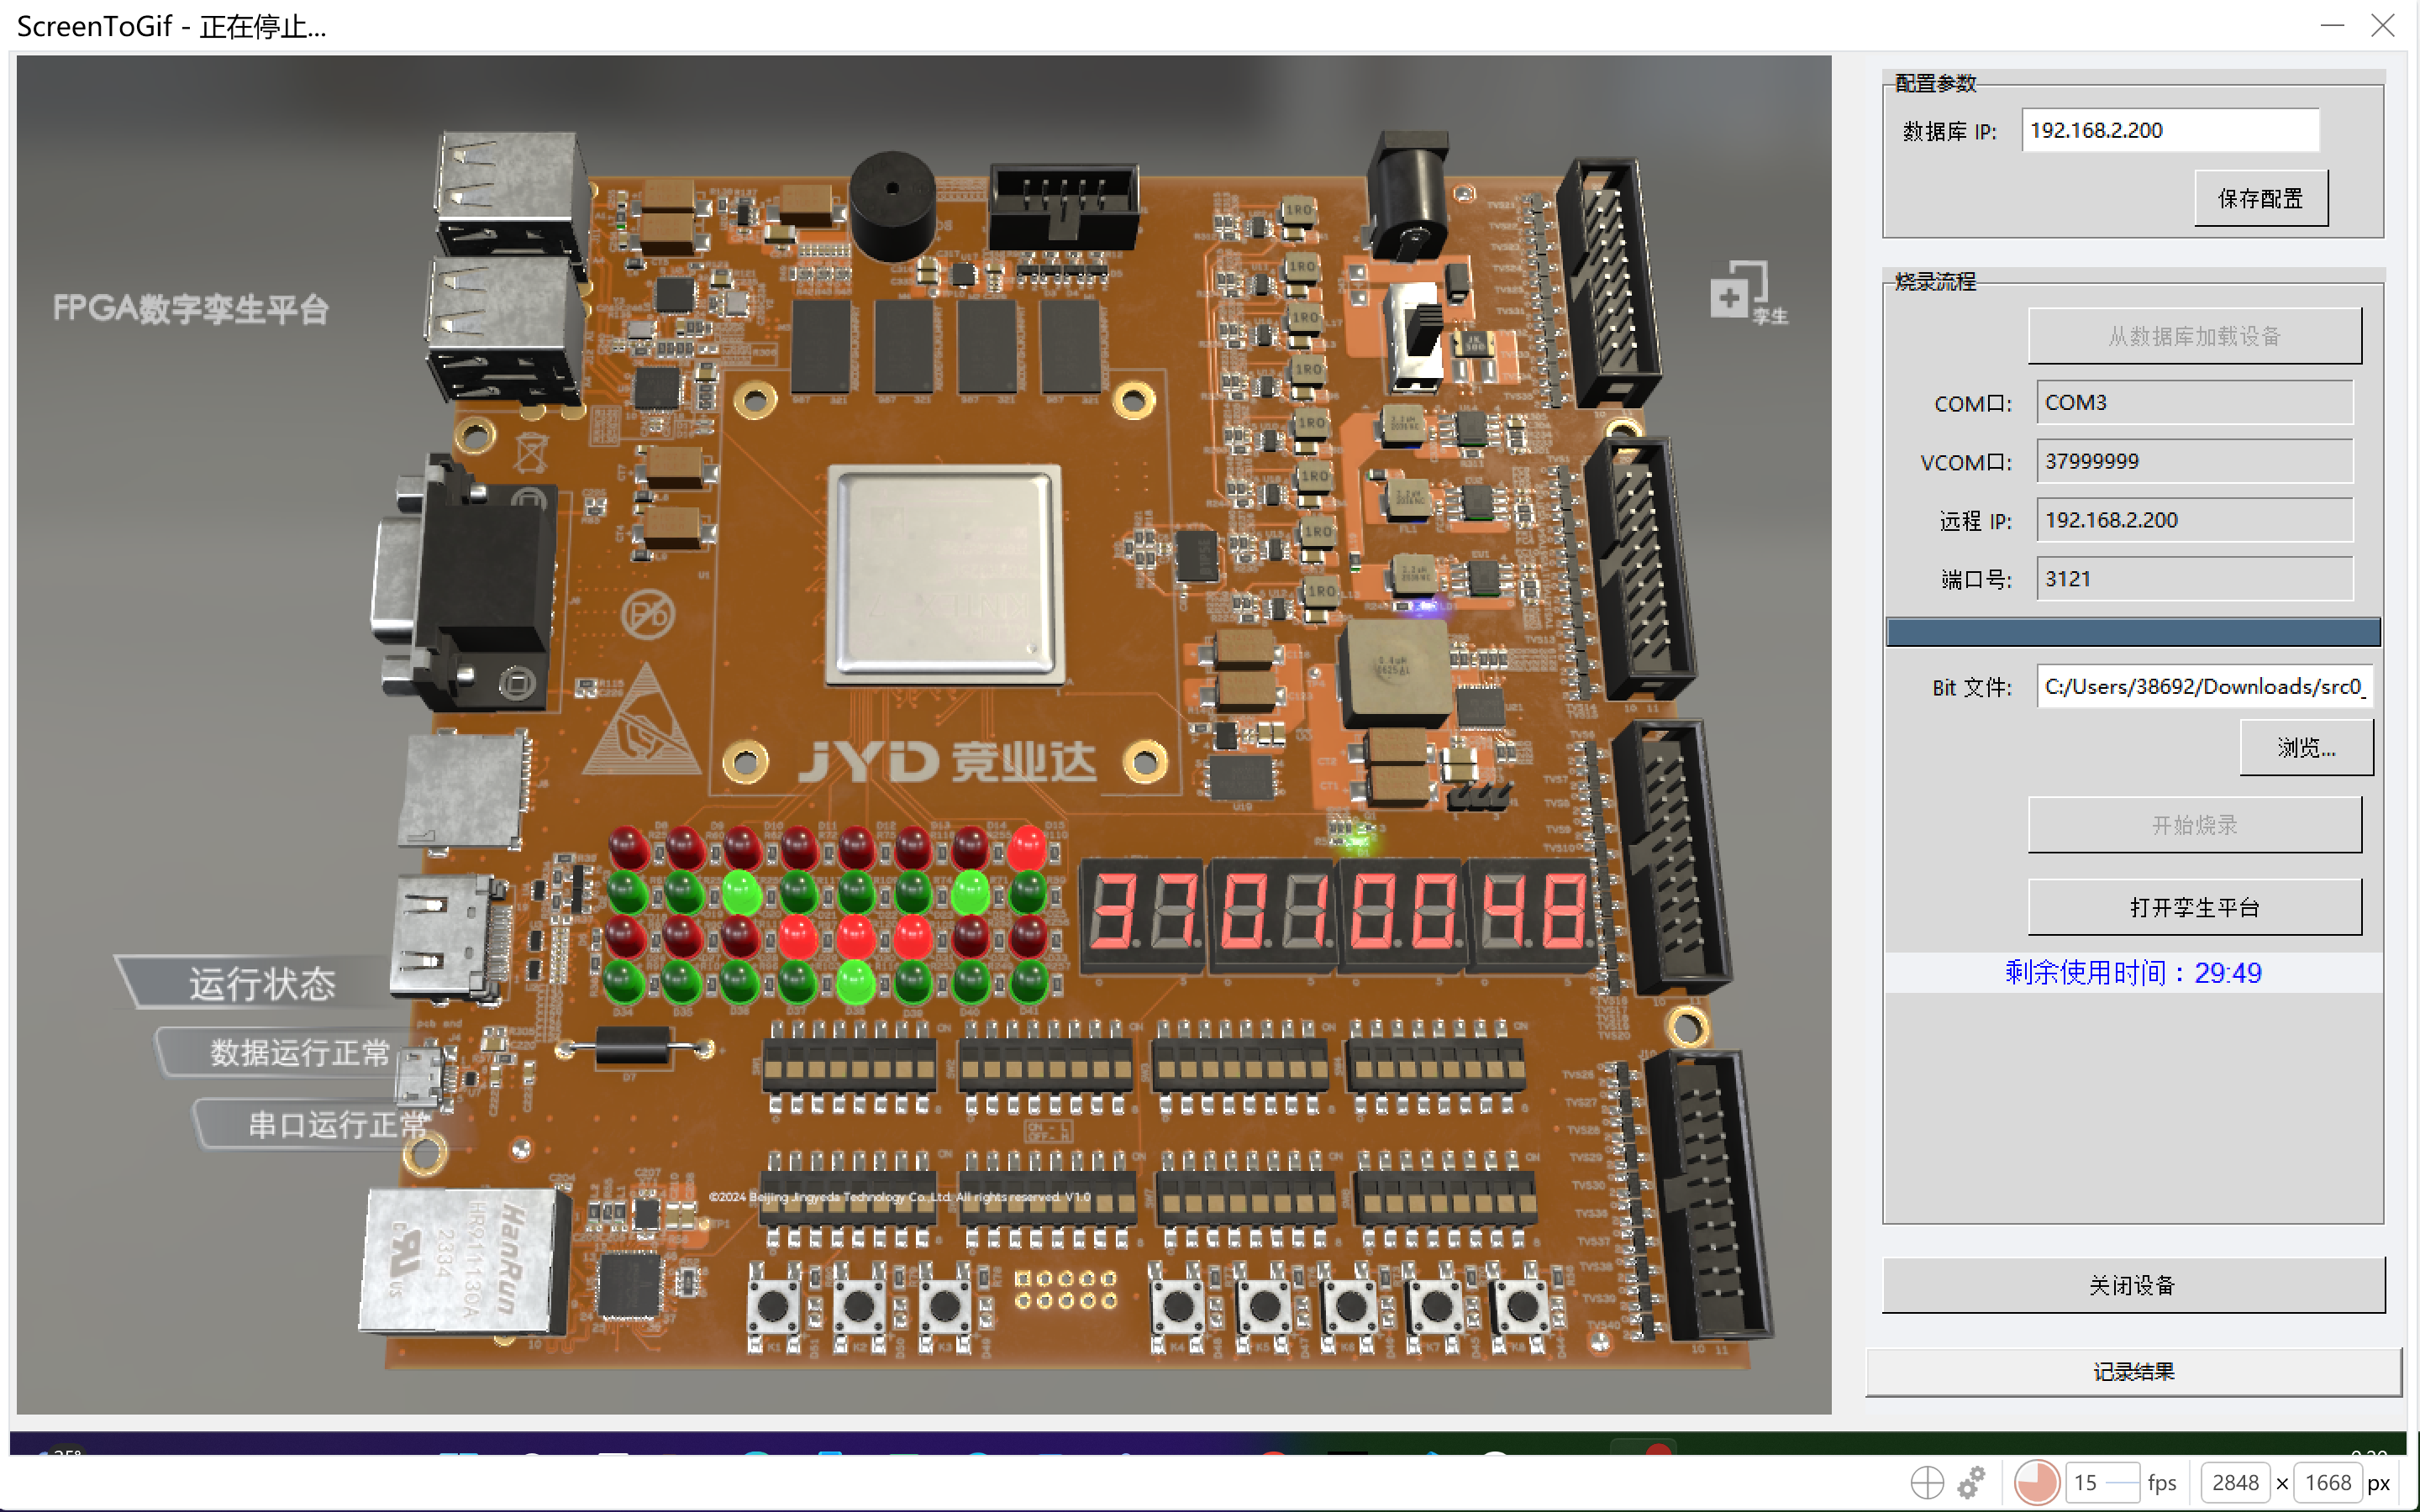
\includegraphics[width=0.95\linewidth]{figures/digital_twin_src0.png}
  \caption{src0 数字孪生运行结果}
  \label{fig:digital-src0-preview}
\end{figure}

\begin{figure}[H]
  \centering
  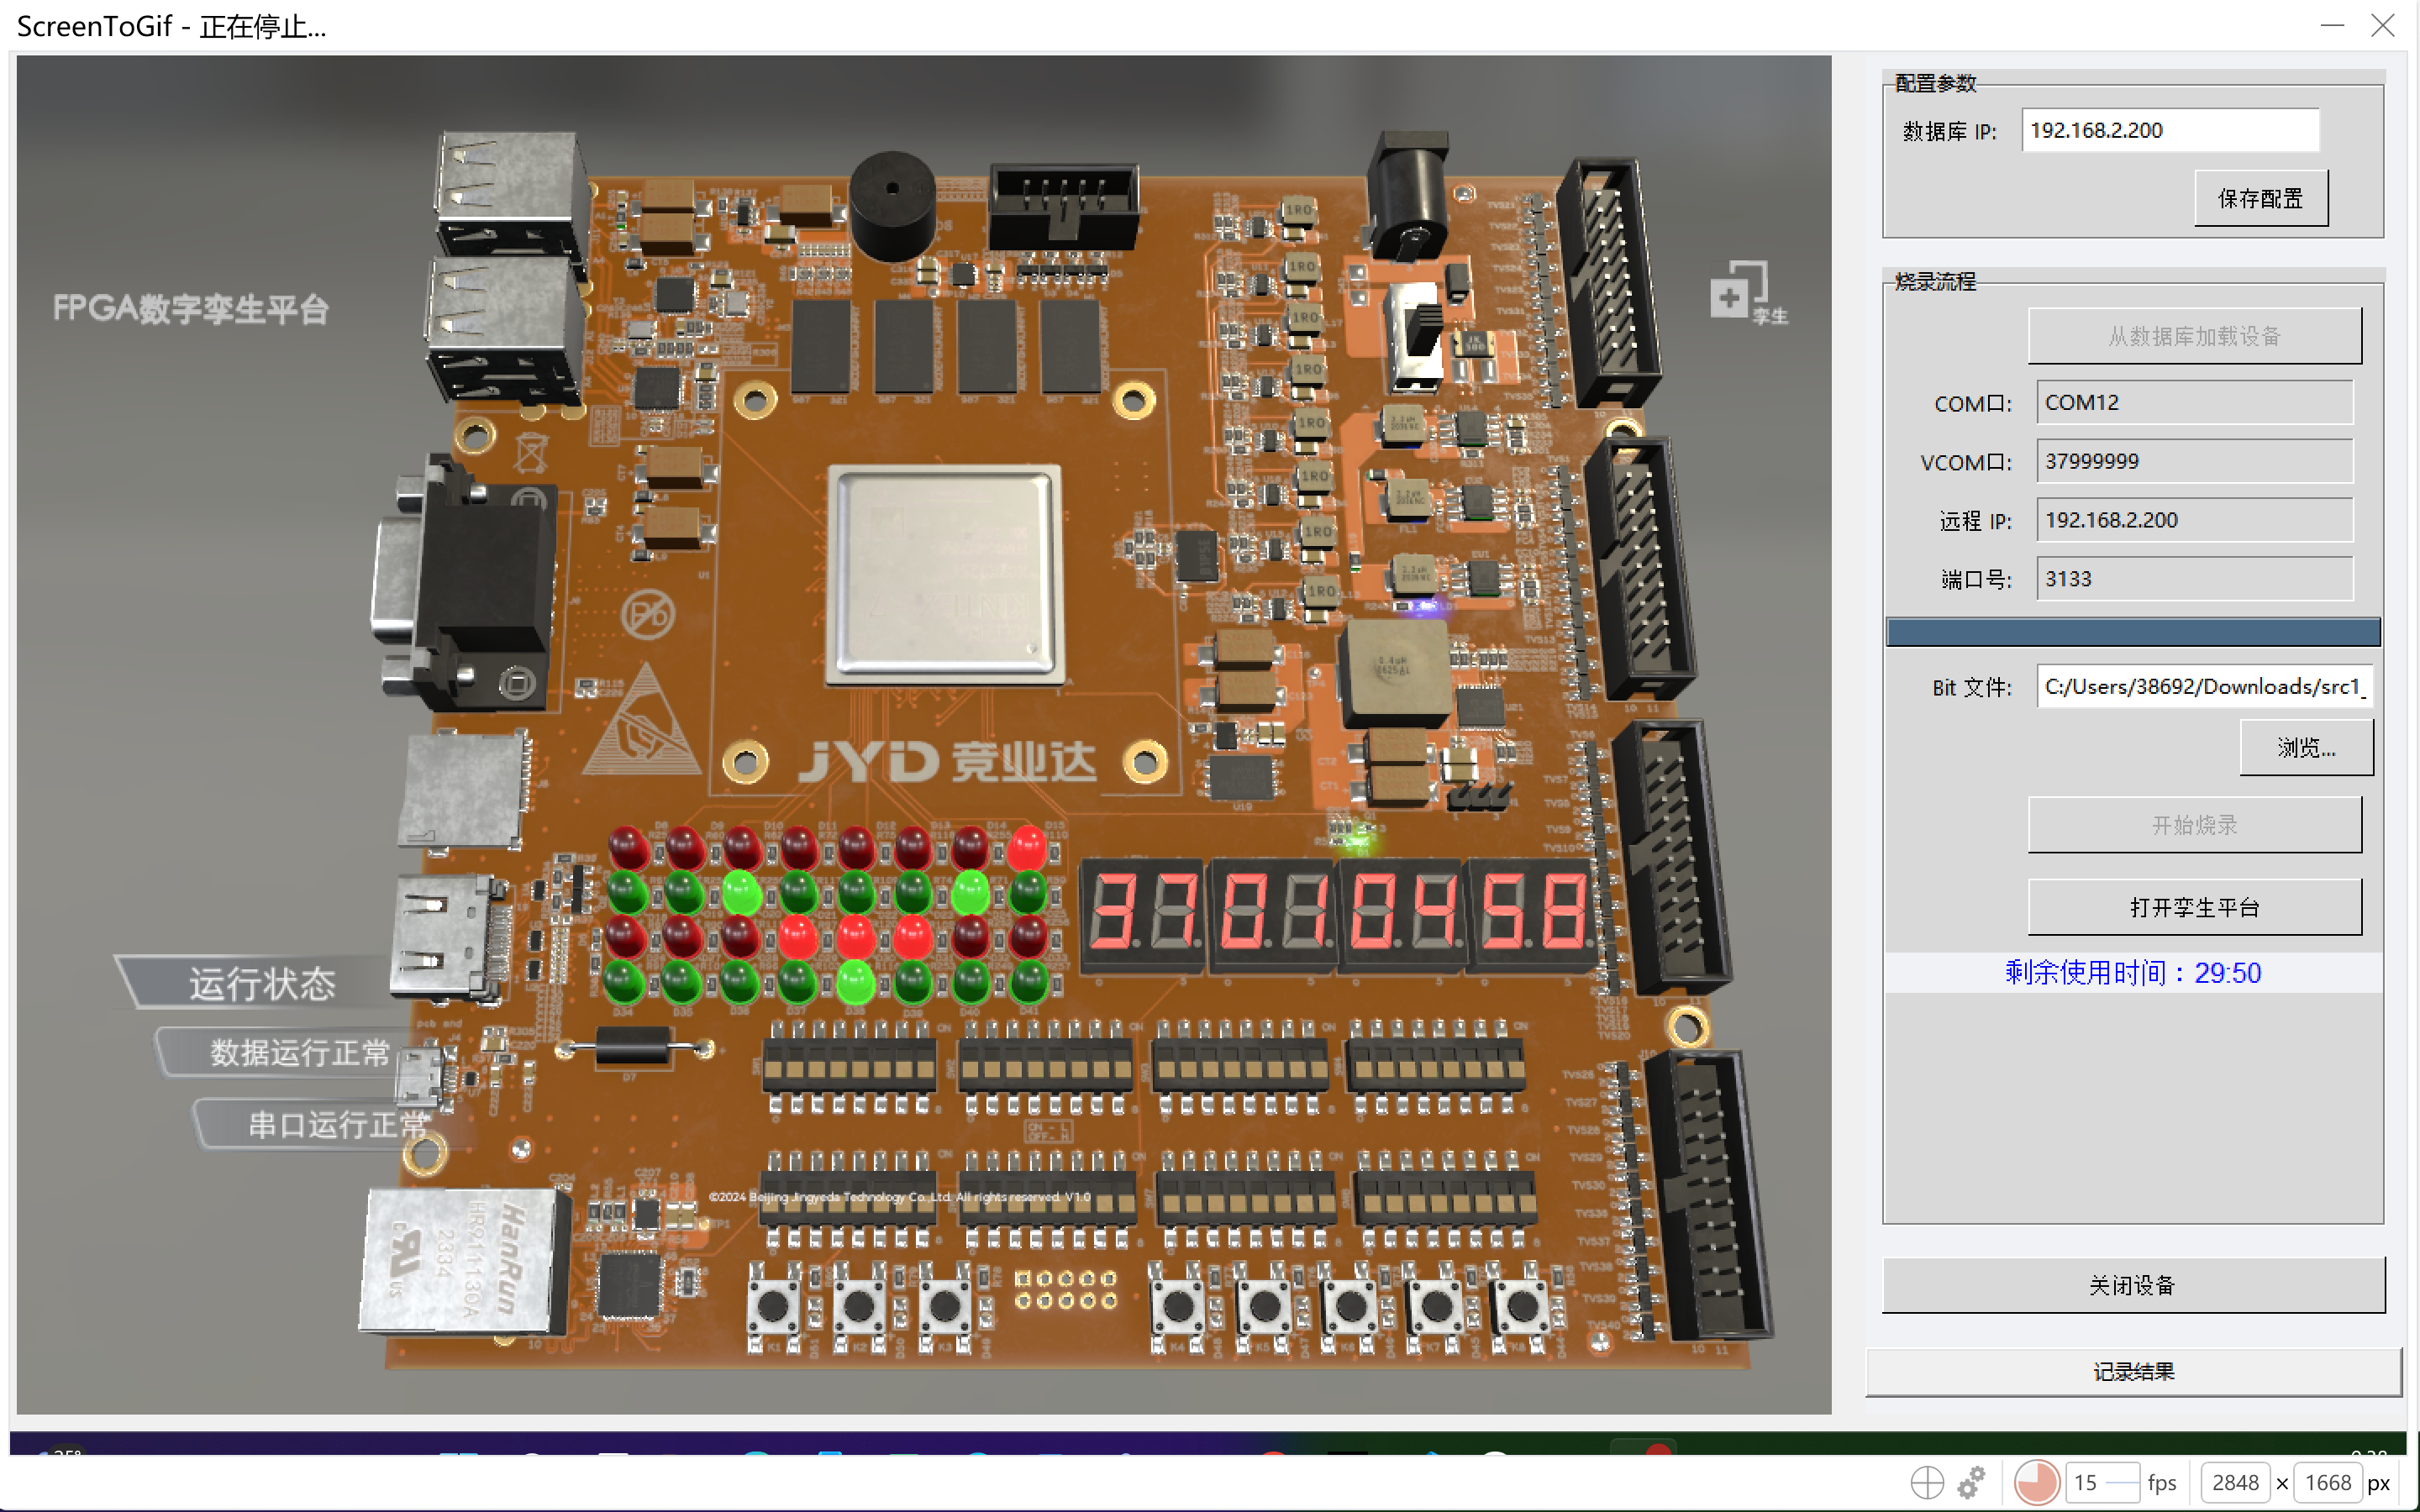
\includegraphics[width=0.95\linewidth]{figures/digital_twin_src1.png}
  \caption{src1 数字孪生运行结果}
  \label{fig:digital-src1-preview}
\end{figure}

\begin{figure}[H]
  \centering
  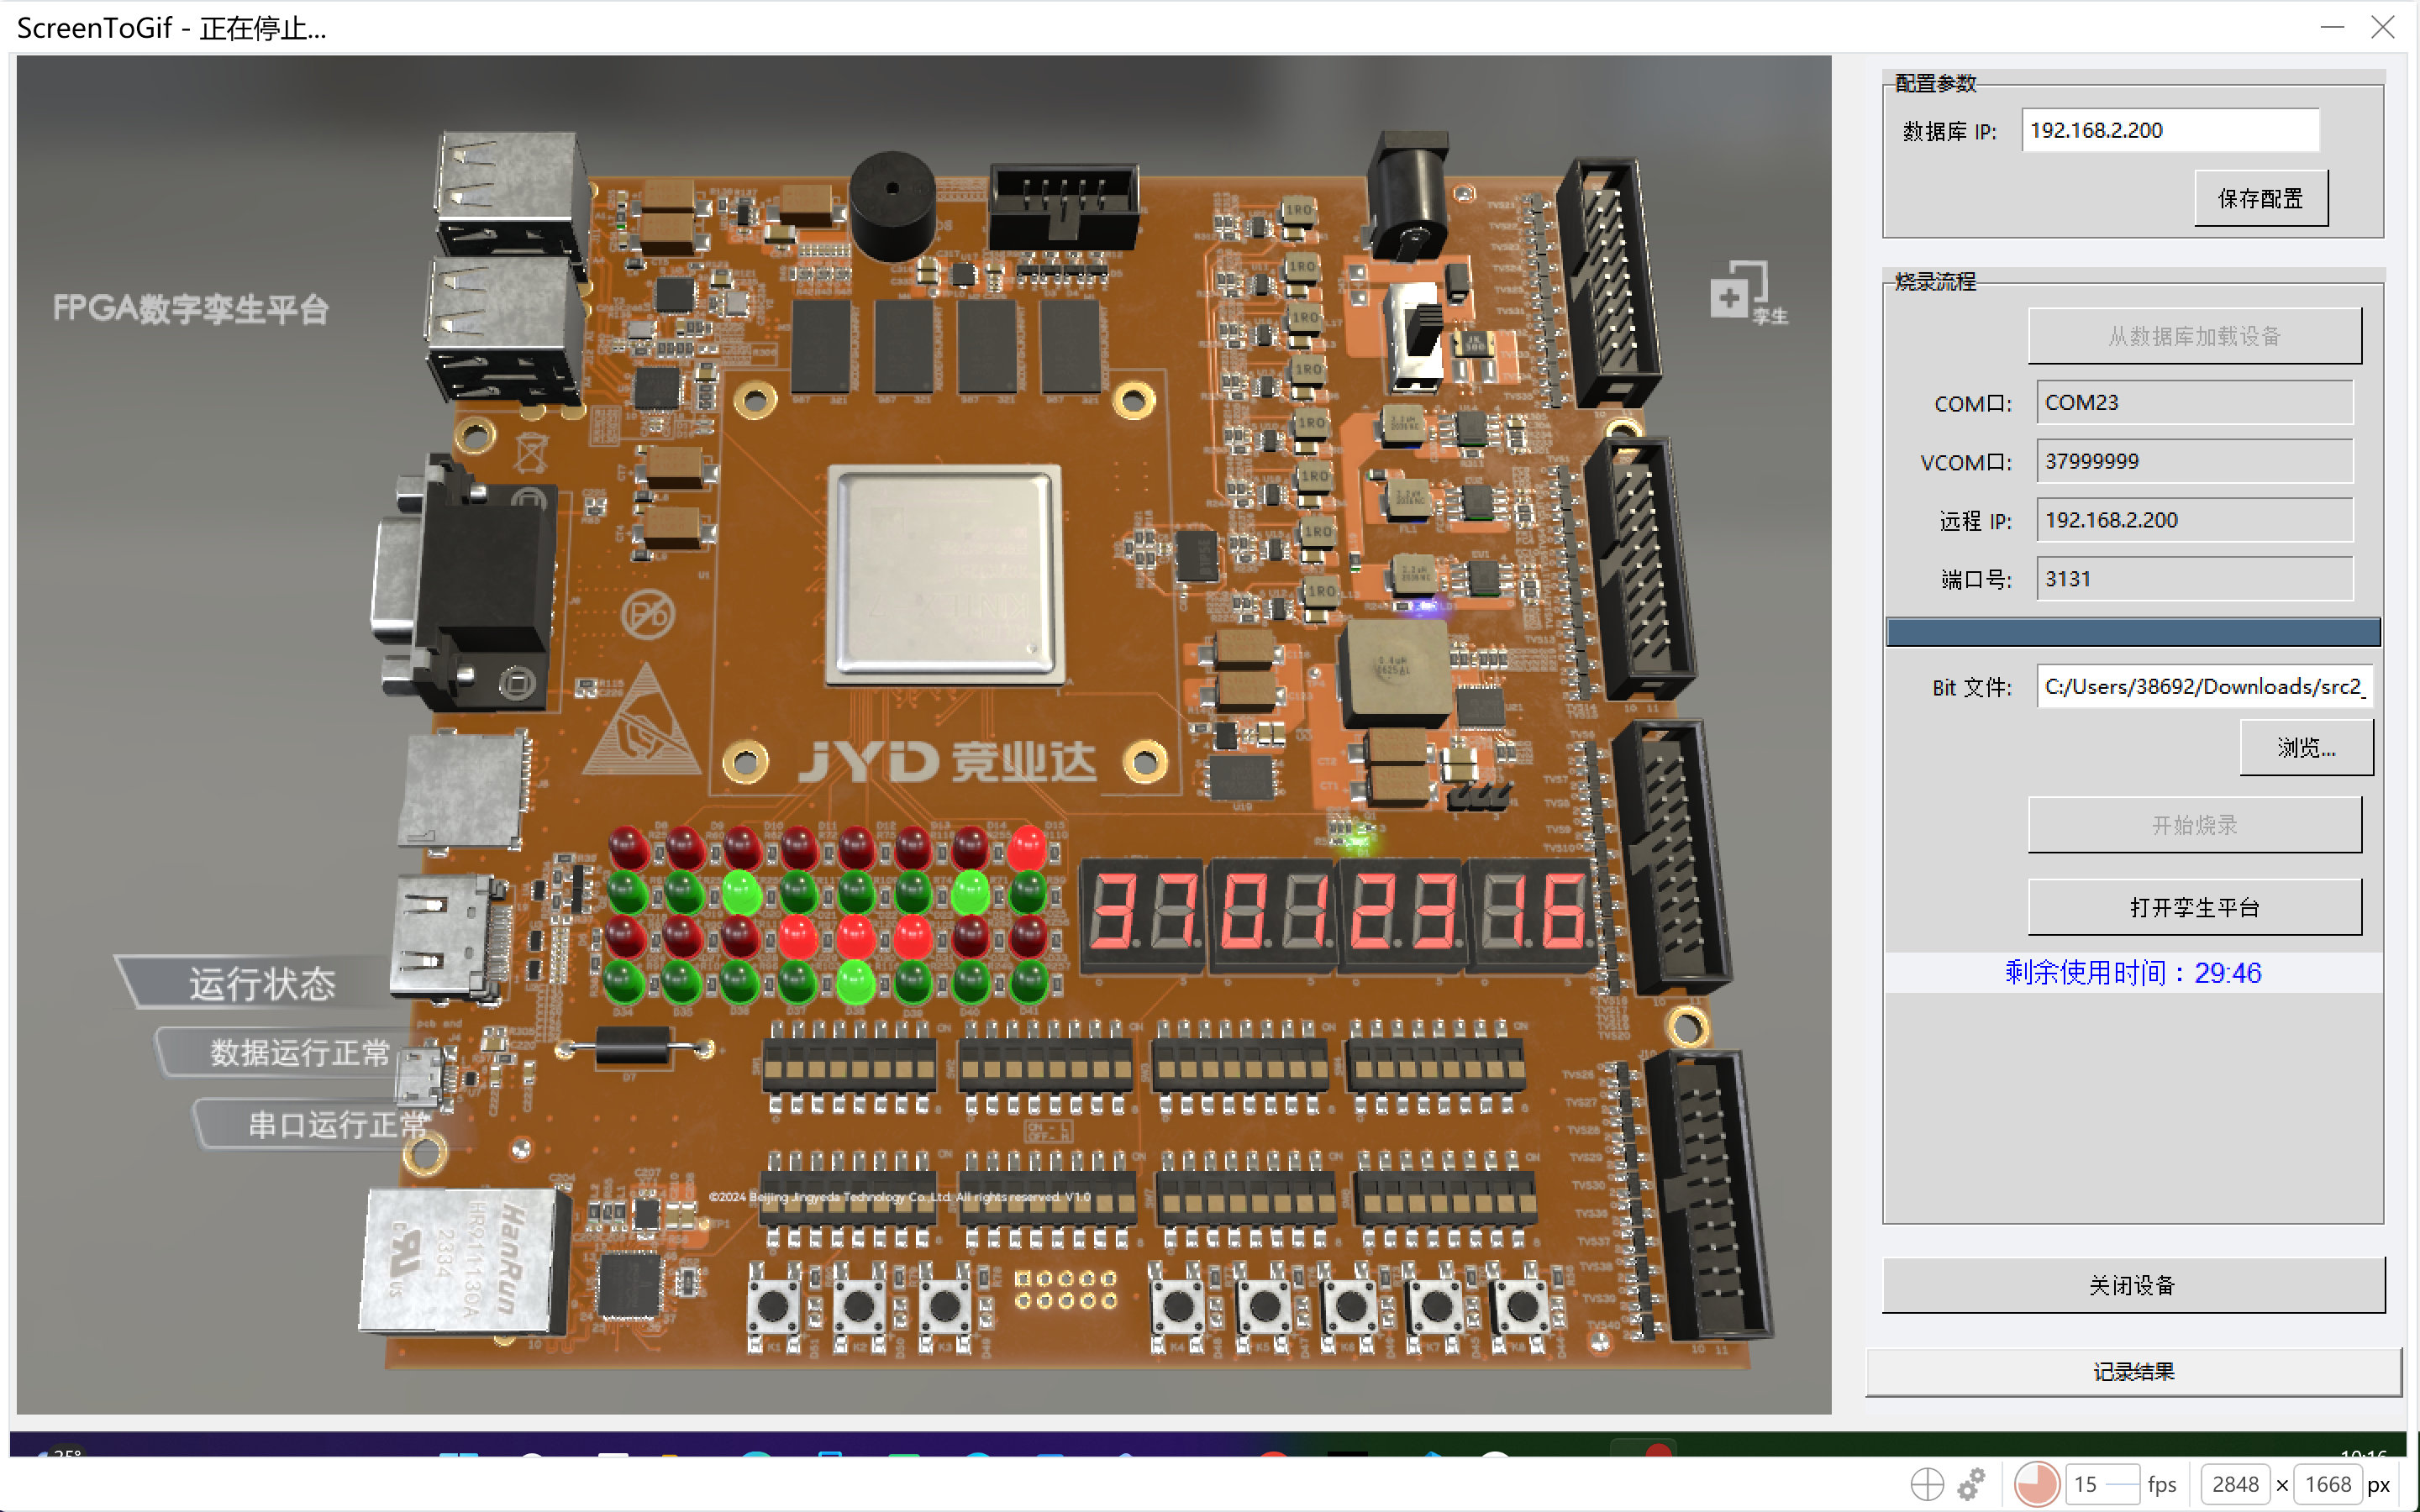
\includegraphics[width=0.95\linewidth]{figures/digital_twin_src2.png}
  \caption{src2 数字孪生运行结果}
  \label{fig:digital-src2-preview}
\end{figure}
\newpage

\begin{center}
  {\zihao{2}\bfseries RISC-V CPU仿真验证报告}\par
\end{center}
\vspace{0.5em}

\section{验证环境}

\subsection{仿真工具}

仿真器版本：Verilator v5.046，GTKWave v3.3.116。

具体使用：使用 Verilator 将硬件电路编译为 C++ 代码，进行高速二值仿真。生成 .fst 波形文件后，可使用波形展示工具 Gtkwave 查看波形。

\subsection{测试环境说明}

\subsubsection{操作系统}

Ubuntu 24.04。

\subsubsection{测试语言}

C++ 结合 Verilog。使用 Verilog 将核心 CPU 模块放入仿真 testbench 中，在 testbench 中结合 Verilator 的 DPI-C 功能调用 C++ 函数，从而实现复杂行为的仿真。

\subsubsection{开发工具链与构建系统}

C++ 编译器：g++ 13.3.0（Ubuntu 13.3.0-6ubuntu2\textasciitilde 24.04）。

RISC-V 工具链：riscv32-unknown-linux-gnu-gcc 14.2.0（g04696df0963）。

\subsubsection{程序运行时环境}

针对赛题的内存空间，本设计编写了专用的链接脚本以及入口函数，为编译程序提供最基本的运行时环境。仿真 RTE 环境的内存空间示意如图~\ref{fig:rte-memory} 所示。

\begin{figure}[H]
  \centering
  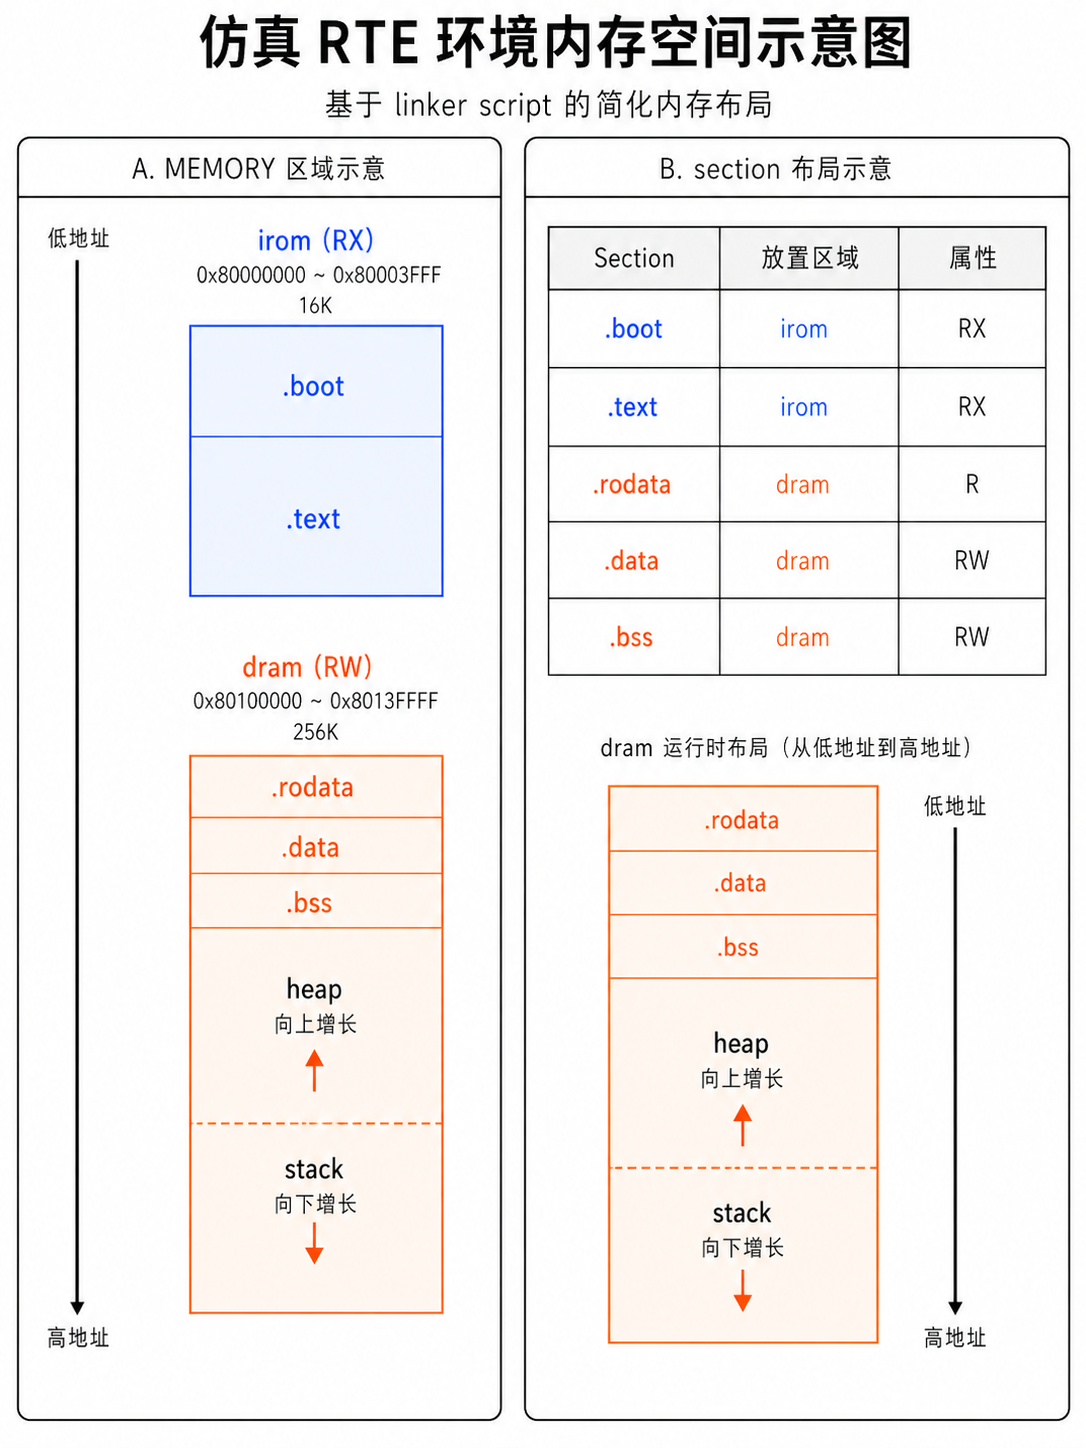
\includegraphics[width=0.82\linewidth]{figures/sim_rte_memory.png}
  \caption{仿真 RTE 环境内存空间示意图}
  \label{fig:rte-memory}
\end{figure}

\section{仿真平台介绍}

\subsection{RV32I 指令集测试}

本小节采用官方开源的 RISC-V 架构测试套件 riscv-tests 中的 rv32ui（User-level Integer）模块作为测试用例，覆盖 RV32I 基础指令集中规定的 37 条指令。测试套件通过验证指令执行后目标寄存器或内存的值是否符合预期，判断该条指令的功能正确性。仿真时，通过 Verilator 加载各指令对应的机器码文件，并根据执行结束后的标志位，例如将特定寄存器置为 Pass/Fail 状态值，判定测试结果。

\subsubsection{算术与逻辑运算指令测试}

测试内容：包含 \code{add}、\code{sub}、\code{and}、\code{or}、\code{xor}、\code{sll}、\code{srl}、\code{sra} 等寄存器-寄存器操作，以及对应的立即数操作（\code{addi}、\code{andi} 等）和 \code{lui}、\code{auipc} 指令。

测试机制：采用 riscv-tests 中的 add.S、addi.S 等独立测试文件。例如，对于 \code{add} 指令，测试程序会自动生成多种边界条件，如正数相加、负数相加、溢出等，并验证写入目标寄存器的结果。

\subsubsection{控制流指令测试}

测试内容：包含无条件跳转指令 \code{jal}、\code{jalr} 和条件分支指令 \code{beq}、\code{bne}、\code{blt}、\code{bge}、\code{bltu}、\code{bgeu}。

测试机制：采用套件中的 jal.S、beq.S 等文件。测试用例会设计特定的跳转网络，若分支条件判断错误或跳转地址计算错误，程序将跳转至预设的 Fail 分支；若全部分支逻辑正确，则最终跳转至 Pass 分支。

\subsubsection{访存指令测试}

测试内容：包含加载指令 \code{lb}、\code{lh}、\code{lw}、\code{lbu}、\code{lhu} 和存储指令 \code{sb}、\code{sh}、\code{sw}。

测试机制：采用套件中的 lw.S、sw.S 等文件。测试程序会先将已知数据通过 Store 指令写入特定内存地址，再通过 Load 指令读取，对比写入与读取的数据是否一致，并验证符号扩展与零扩展逻辑是否正确。

\subsection{RV32I CPU 性能测试}

本节采用业界公认的微处理器性能评估基准程序 CoreMark，对自研 RV32I 流水线处理器的架构性能以及综合运算能力进行量化测试。

\subsubsection{CoreMark 移植与 RTE 协同配置}

为了在裸机仿真环境中运行复杂的 CoreMark 算法，本测试将 CoreMark 源码与自主编写的运行时环境（RTE）进行了深度整合与共同编译。RTE 在此处承担关键的软硬件适配工作。

自校验与退出验证：CoreMark 包含列表处理、矩阵运算、状态机和 CRC 校验等模块。在所有算法迭代完成后，CoreMark 会进行严格的内部数据一致性校验。校验通过后，RTE 将引导处理器执行正常退出流程并返回 0；若校验失败，则返回 1。Verilator 测试平台据此判断该次性能评估是否有效。

\subsubsection{CoreMark 仿真环境测试用例}

编译与优化配置：使用 RISC-V 交叉编译工具链对集成 RTE 的 CoreMark 源码进行编译，测试用例中明确开启特定优化等级 -O2，并指定对应的微架构参数，以充分评估处理器流水线性能。

仿真验证过程：将编译出的固件加载至 Verilator 仿真的指令/数据存储器模型中，复位 Mundus 处理器后开始执行。仿真平台持续运行，直至捕获到 RTE 传递的返回值 0。此时，提取程序运行期间打印出的或存储在特定内存地址的总时钟周期数，结合仿真的目标频率，用于统计 CoreMark 程序在本处理器上的运行周期数、guest 指令数和 IPC 等性能指标。

\subsection{RV32I CPU 其它测试}

\subsubsection{BPU（分支预测模块）测试}

为了保证 BPU 实现的正确性，目前采用 RTL 代码和 C++ 模拟代码相互验证的方式。目前分支预测采用两位饱和计数器，并使用 Branch Target Buffer 记录历史跳转目标地址。

在取指阶段，通过 DPI-C 的方式将 RTL 的 fetch\_pc、predicted\_pc 和 predicted\_taken 传给参考模型。参考模型使用相同的 bimodal 算法对该 PC 进行预测，并与 RTL 输出进行比较。比较内容包括：（1）方向预测是否一致，即 taken/not-taken 是否相同；（2）若预测 taken，则目标地址是否一致；（3）对于发生流水线重定向的取指事件，不参与 fetch-side 对比，避免将 flush 后的无效预测计入统计。

在执行阶段，当 RTL 中的更新信号拉高时，将真实分支结果传给参考模型，包括更新时该条分支指令的 PC 地址、真实跳转的目标地址和真实是否跳转的结果。参考模型使用这些信息更新自身状态，从而确保更新过程的同步性。

\section{仿真结果}

\subsection{RV32I 指令集测试结果}

\subsubsection{riscv-tests 测试结果}

riscv-tests 测试结果如图~\ref{fig:riscv-tests-pass} 所示。测试输出中各条 RV32I 指令对应的测试项均显示为 PASS，说明 CPU 对基础整数指令集的功能支持能够通过当前测试套件验证。

\begin{figure}[H]
  \centering
  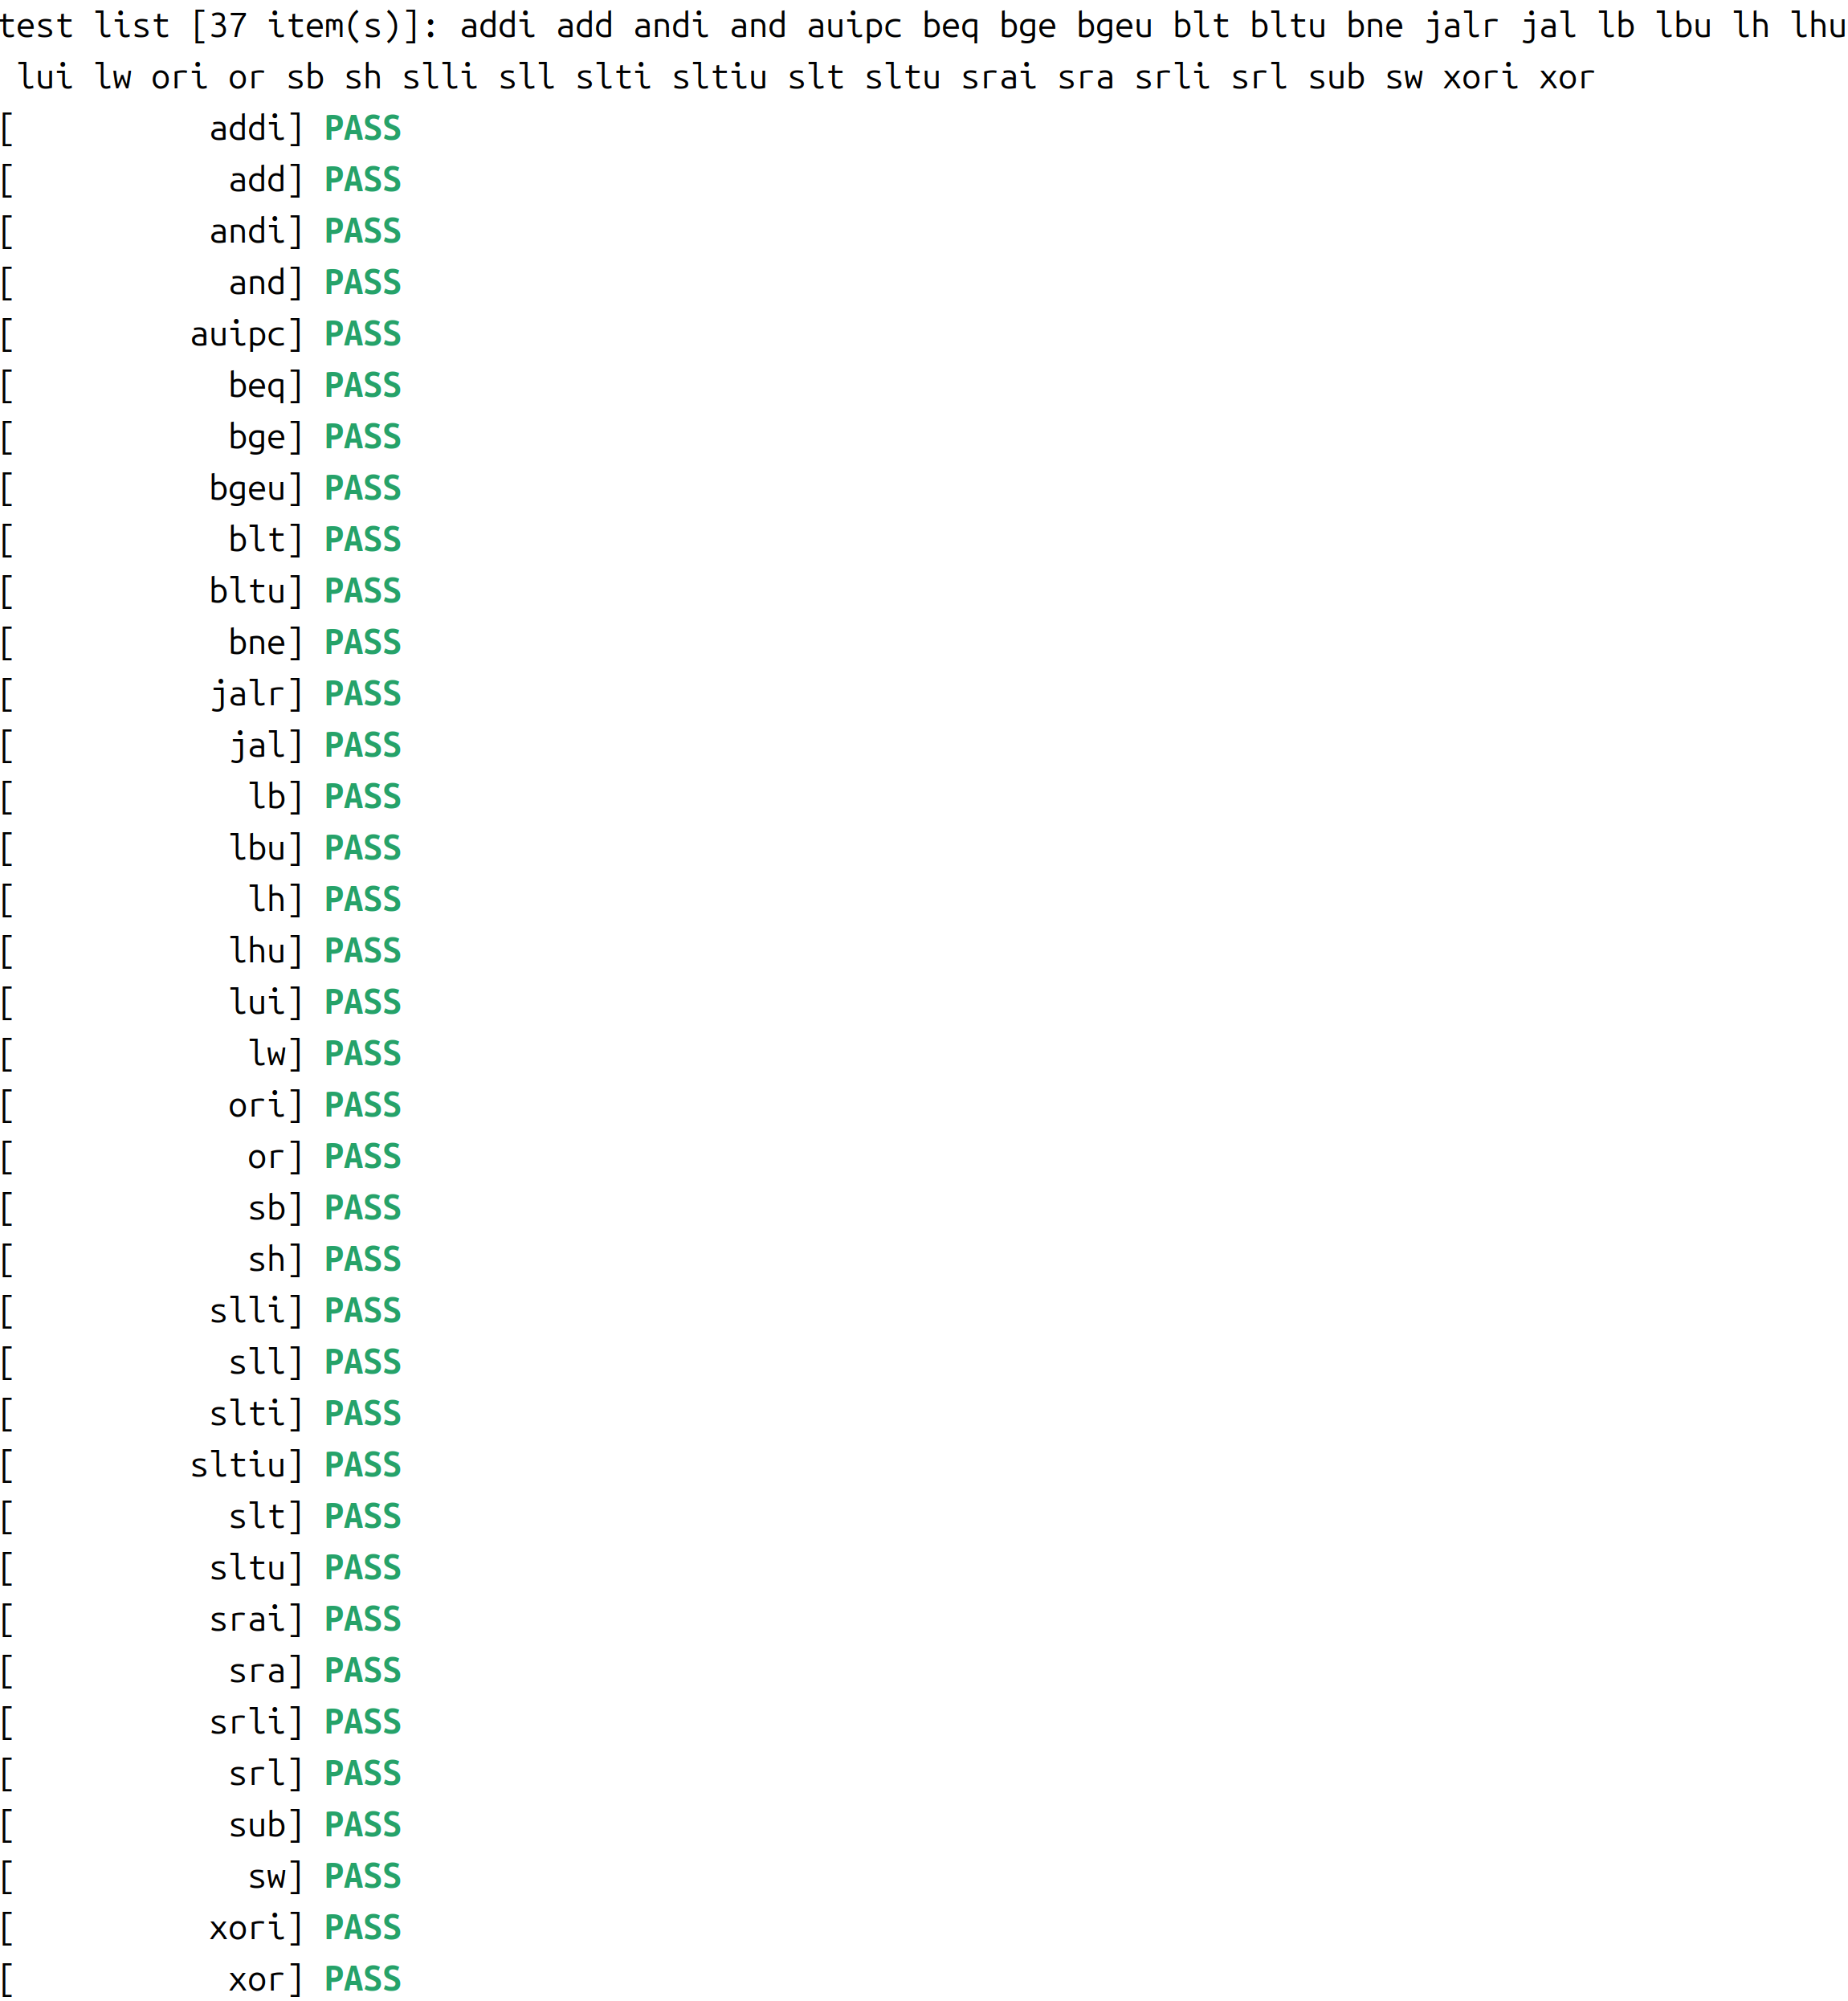
\includegraphics[width=0.90\linewidth]{figures/riscv_tests_pass.png}
  \caption{riscv-tests 指令集测试通过结果}
  \label{fig:riscv-tests-pass}
\end{figure}

\subsection{RV32I CPU 性能测试结果}

\subsubsection{CoreMark 测试结果}

CoreMark 测试结果汇总如表~\ref{tab:coremark-result} 所示，仿真日志截图见图~\ref{fig:coremark-result-bimodal} 和图~\ref{fig:coremark-result-ntk}。两种分支预测策略下程序均命中正常退出条件 HIT GOOD TRAP，说明 CoreMark 程序能够在当前处理器仿真环境中完成有效运行。由于两组测试的 guest 指令数相同，因此可以直接比较总周期数、IPC 和仿真执行效率。

\begin{table}[H]
  \centering
  \caption{CoreMark 仿真性能统计结果}
  \label{tab:coremark-result}
  \renewcommand{\arraystretch}{1.15}
  \begin{normaltable}
  \resizebox{0.70\linewidth}{!}{%
  \begin{tabular}{@{}lccc@{}}
    \toprule
    指标 & Always Not Taken & Bimodal & 变化情况 \\
    \midrule
    主机运行耗时 / us & 173,597,518 & 158,015,344 & 减少 15,582,174 \\
    CPU 总周期数 & 1,097,568,112 & 920,022,264 & 减少 177,545,848 \\
    Guest 指令数 & 747,104,142 & 747,104,142 & 相同 \\
    IPC & 0.680690 & 0.812050 & 提升约 19.30\% \\
    仿真频率 / inst/s & 4,303,656 & 4,728,048 & 提升约 9.86\% \\
    \bottomrule
  \end{tabular}
  }
  \end{normaltable}
\end{table}

\begin{figure}[H]
  \centering
  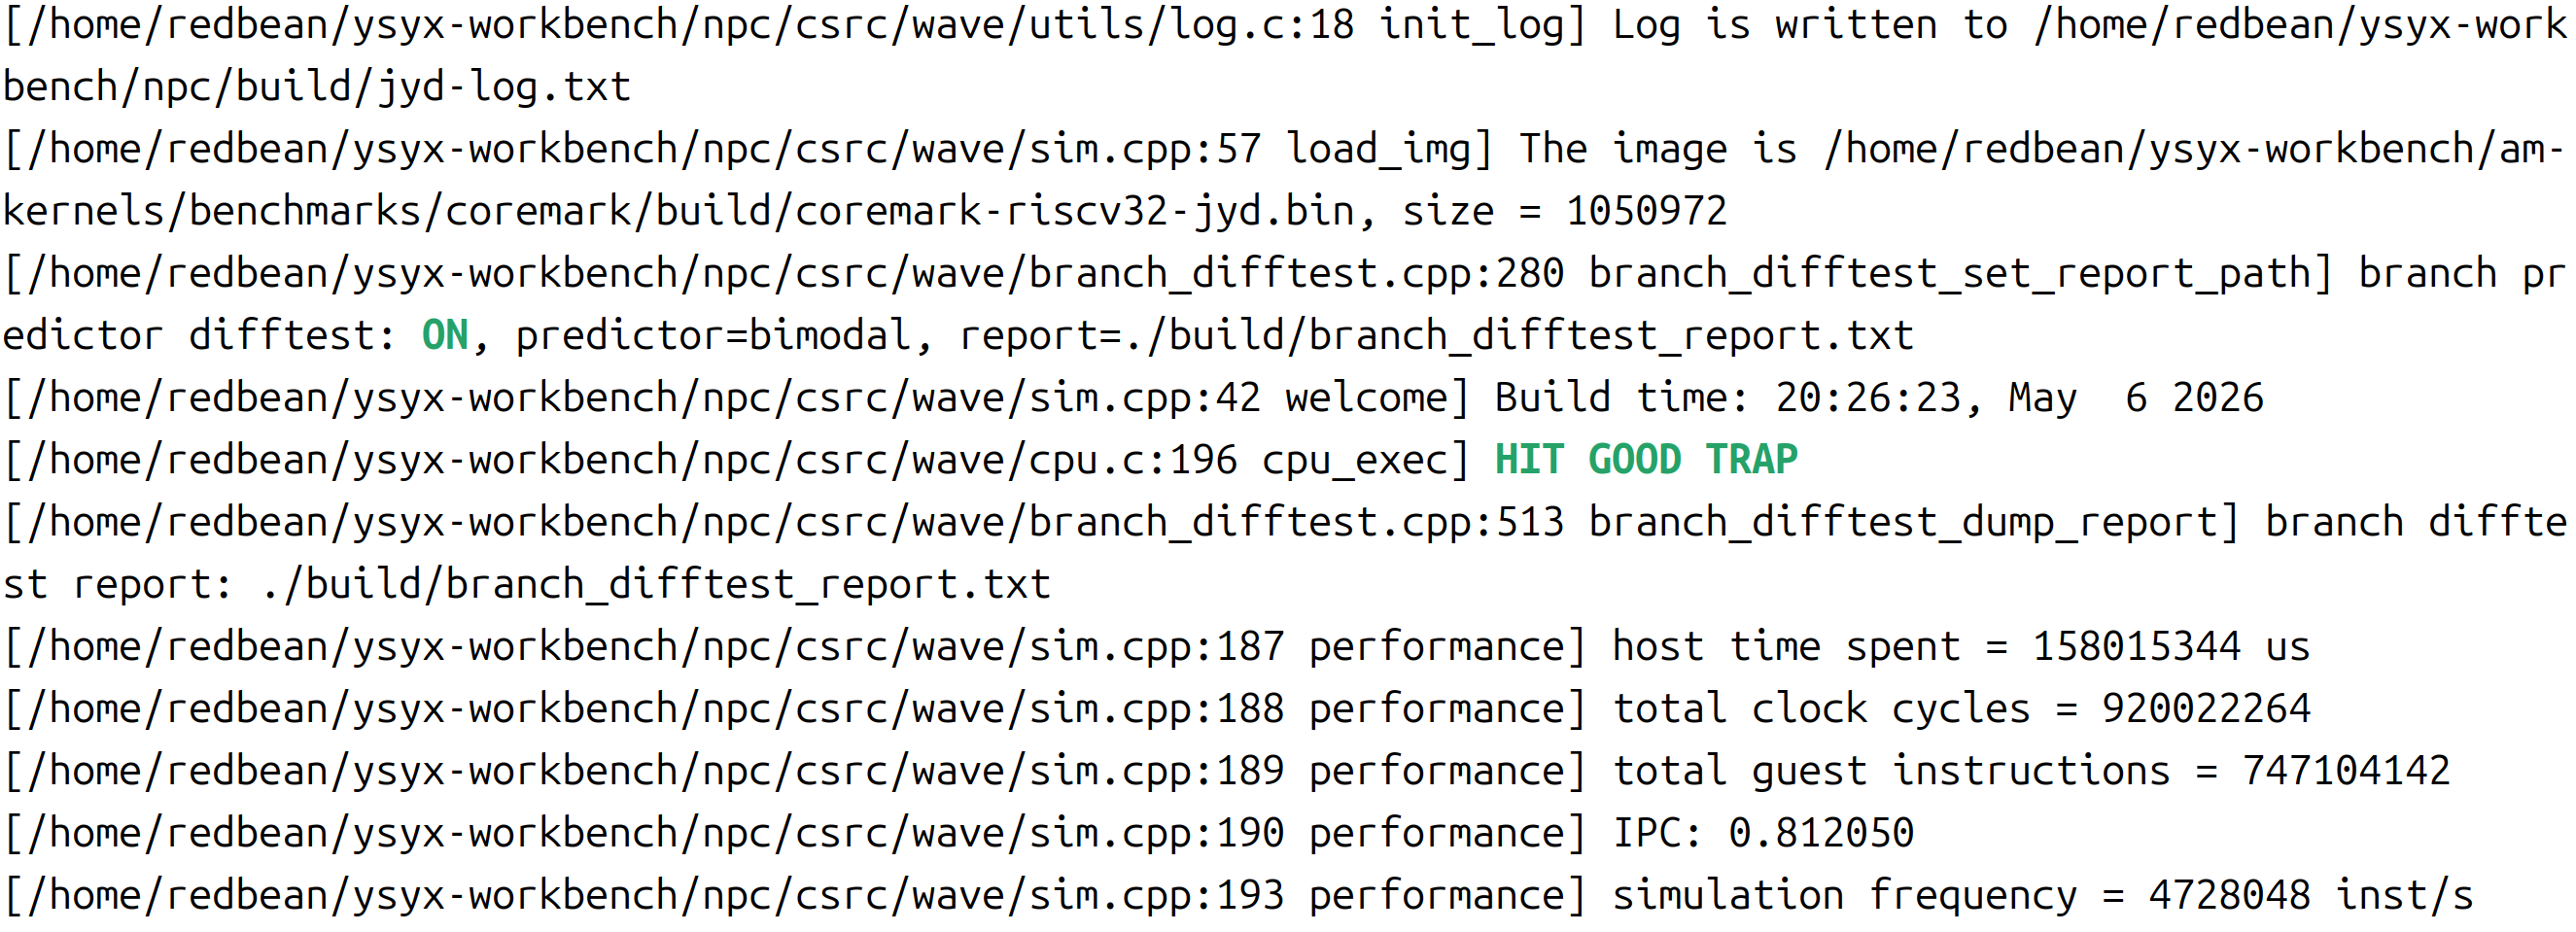
\includegraphics[width=1.0\linewidth]{figures/coremark_result.png}
  \caption{CoreMark 性能测试结果（Bimodal）}
  \label{fig:coremark-result-bimodal}
\end{figure}

\begin{figure}[H]
  \centering
  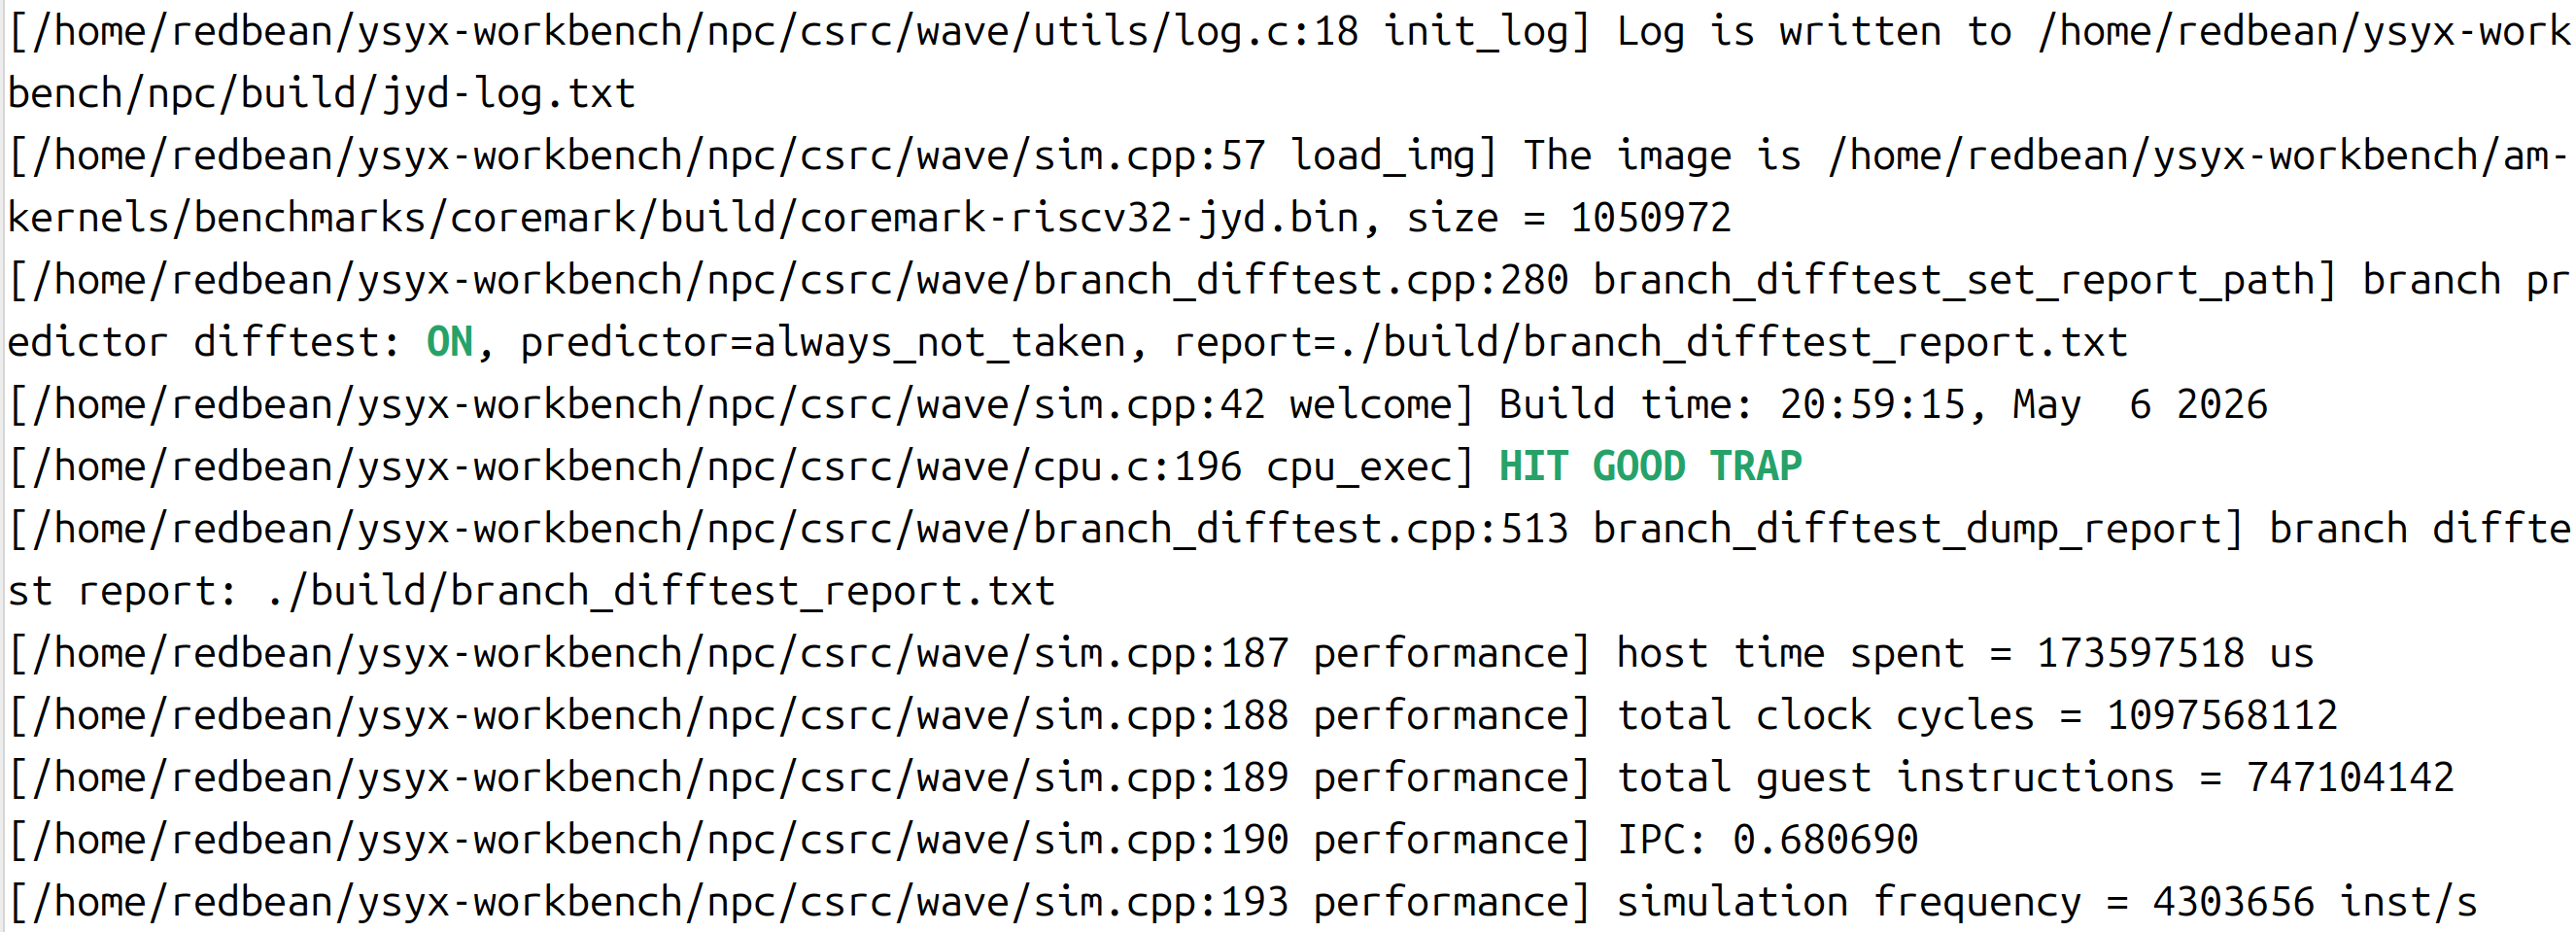
\includegraphics[width=1.0\linewidth]{figures/coremark_ntk.png}
  \caption{CoreMark 性能测试结果（Always Not Taken）}
  \label{fig:coremark-result-ntk}
\end{figure}

\subsection{BPU 测试结果}

从图~\ref{fig:ntk_pass} 和图~\ref{fig:bimodal_pass} 中可以看出，C++ 参考模型与 RTL 实现的 BPU 模块在 fetch-side 对比中的匹配率达到 100\%，说明 RTL 的分支预测方向和目标地址输出与参考模型保持一致，BPU 的基本预测逻辑和更新逻辑能够正确工作。

同时，我们基于 CoreMark 程序对 Always Not Taken 和 Bimodal 两种分支预测策略进行了对比测试。结果表明，引入 Bimodal 预测器后，总预测准确率由 33.65\% 提升至 70.75\%，其中条件分支预测准确率由 37.79\% 提升至 70.26\%，跳转指令预测准确率由 0.00\% 提升至 74.72\%。根据预测正确次数估算，mispredict 次数由约 151.09M 次降低至约 66.60M 次，减少约 84.50M 次；同时，fetch\_redirected\_ignored 由 151,092,422 次降低至 62,259,999 次，说明错误路径取指和流水线冲刷次数明显减少。

从整体性能来看，结合表~\ref{tab:coremark-result} 可知，在 guest 指令数相同的情况下，Bimodal 策略下的总周期数由 1,097,568,112 降低至 920,022,264，减少 177,545,848 个周期；IPC 由 0.680690 提升至 0.812050，提升约 19.30\%。由此可见，Bimodal 分支预测器能够有效学习分支和跳转指令的历史行为，减少控制冒险带来的无效执行开销，从而提升 CPU 整体运行性能。

\begin{figure}[H]
  \centering
  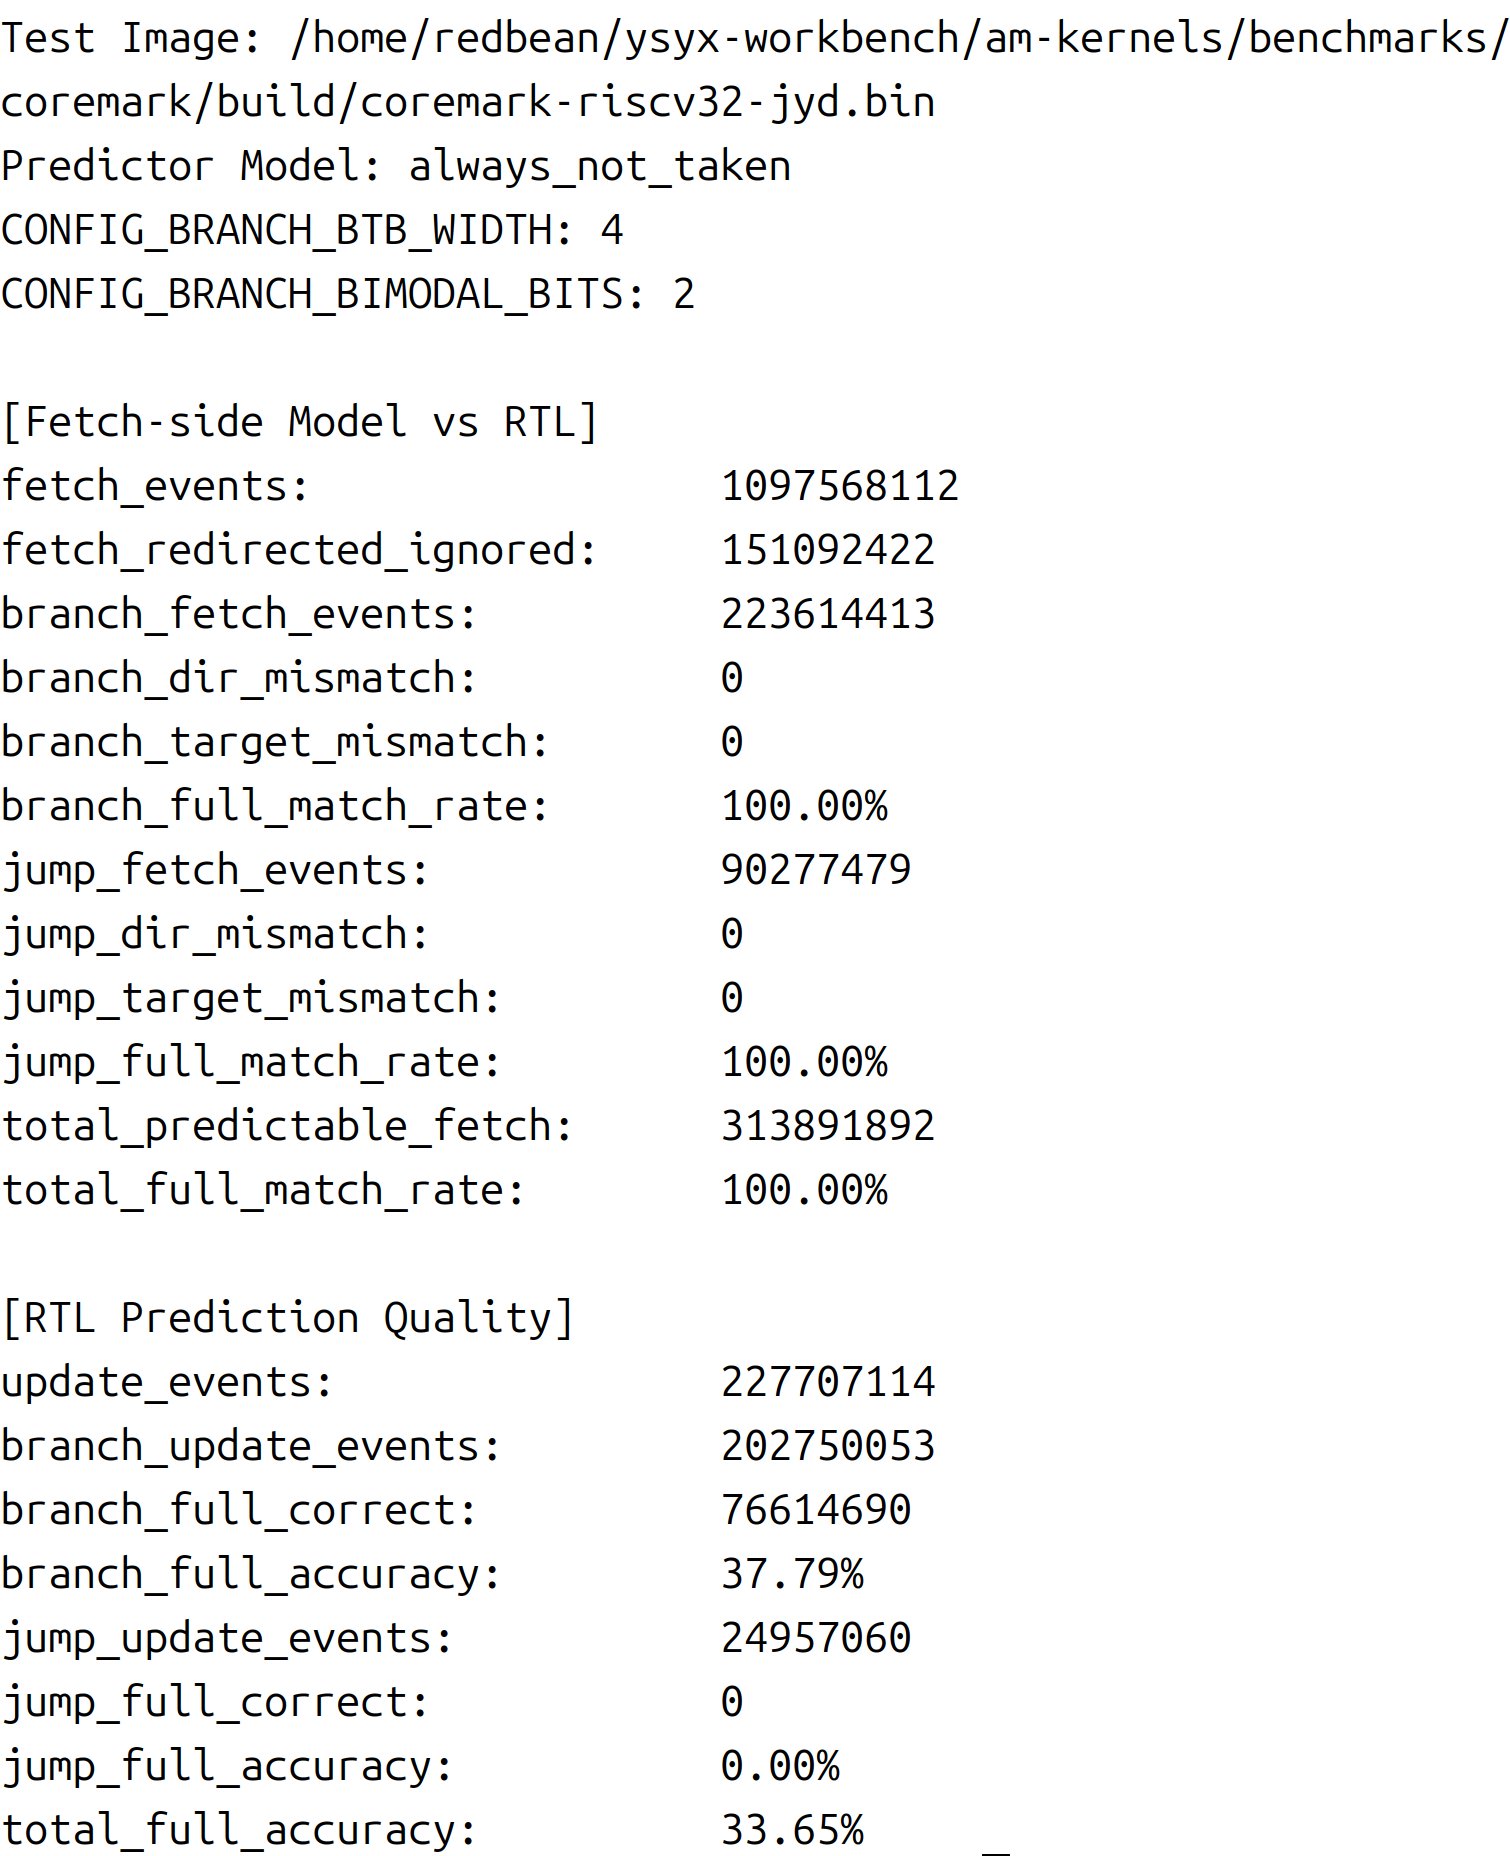
\includegraphics[width=0.90\linewidth]{figures/ntk_sim.png}
  \caption{BPU 测试结果（Always Not Taken）}
  \label{fig:ntk_pass}
\end{figure}

\begin{figure}[H]
  \centering
  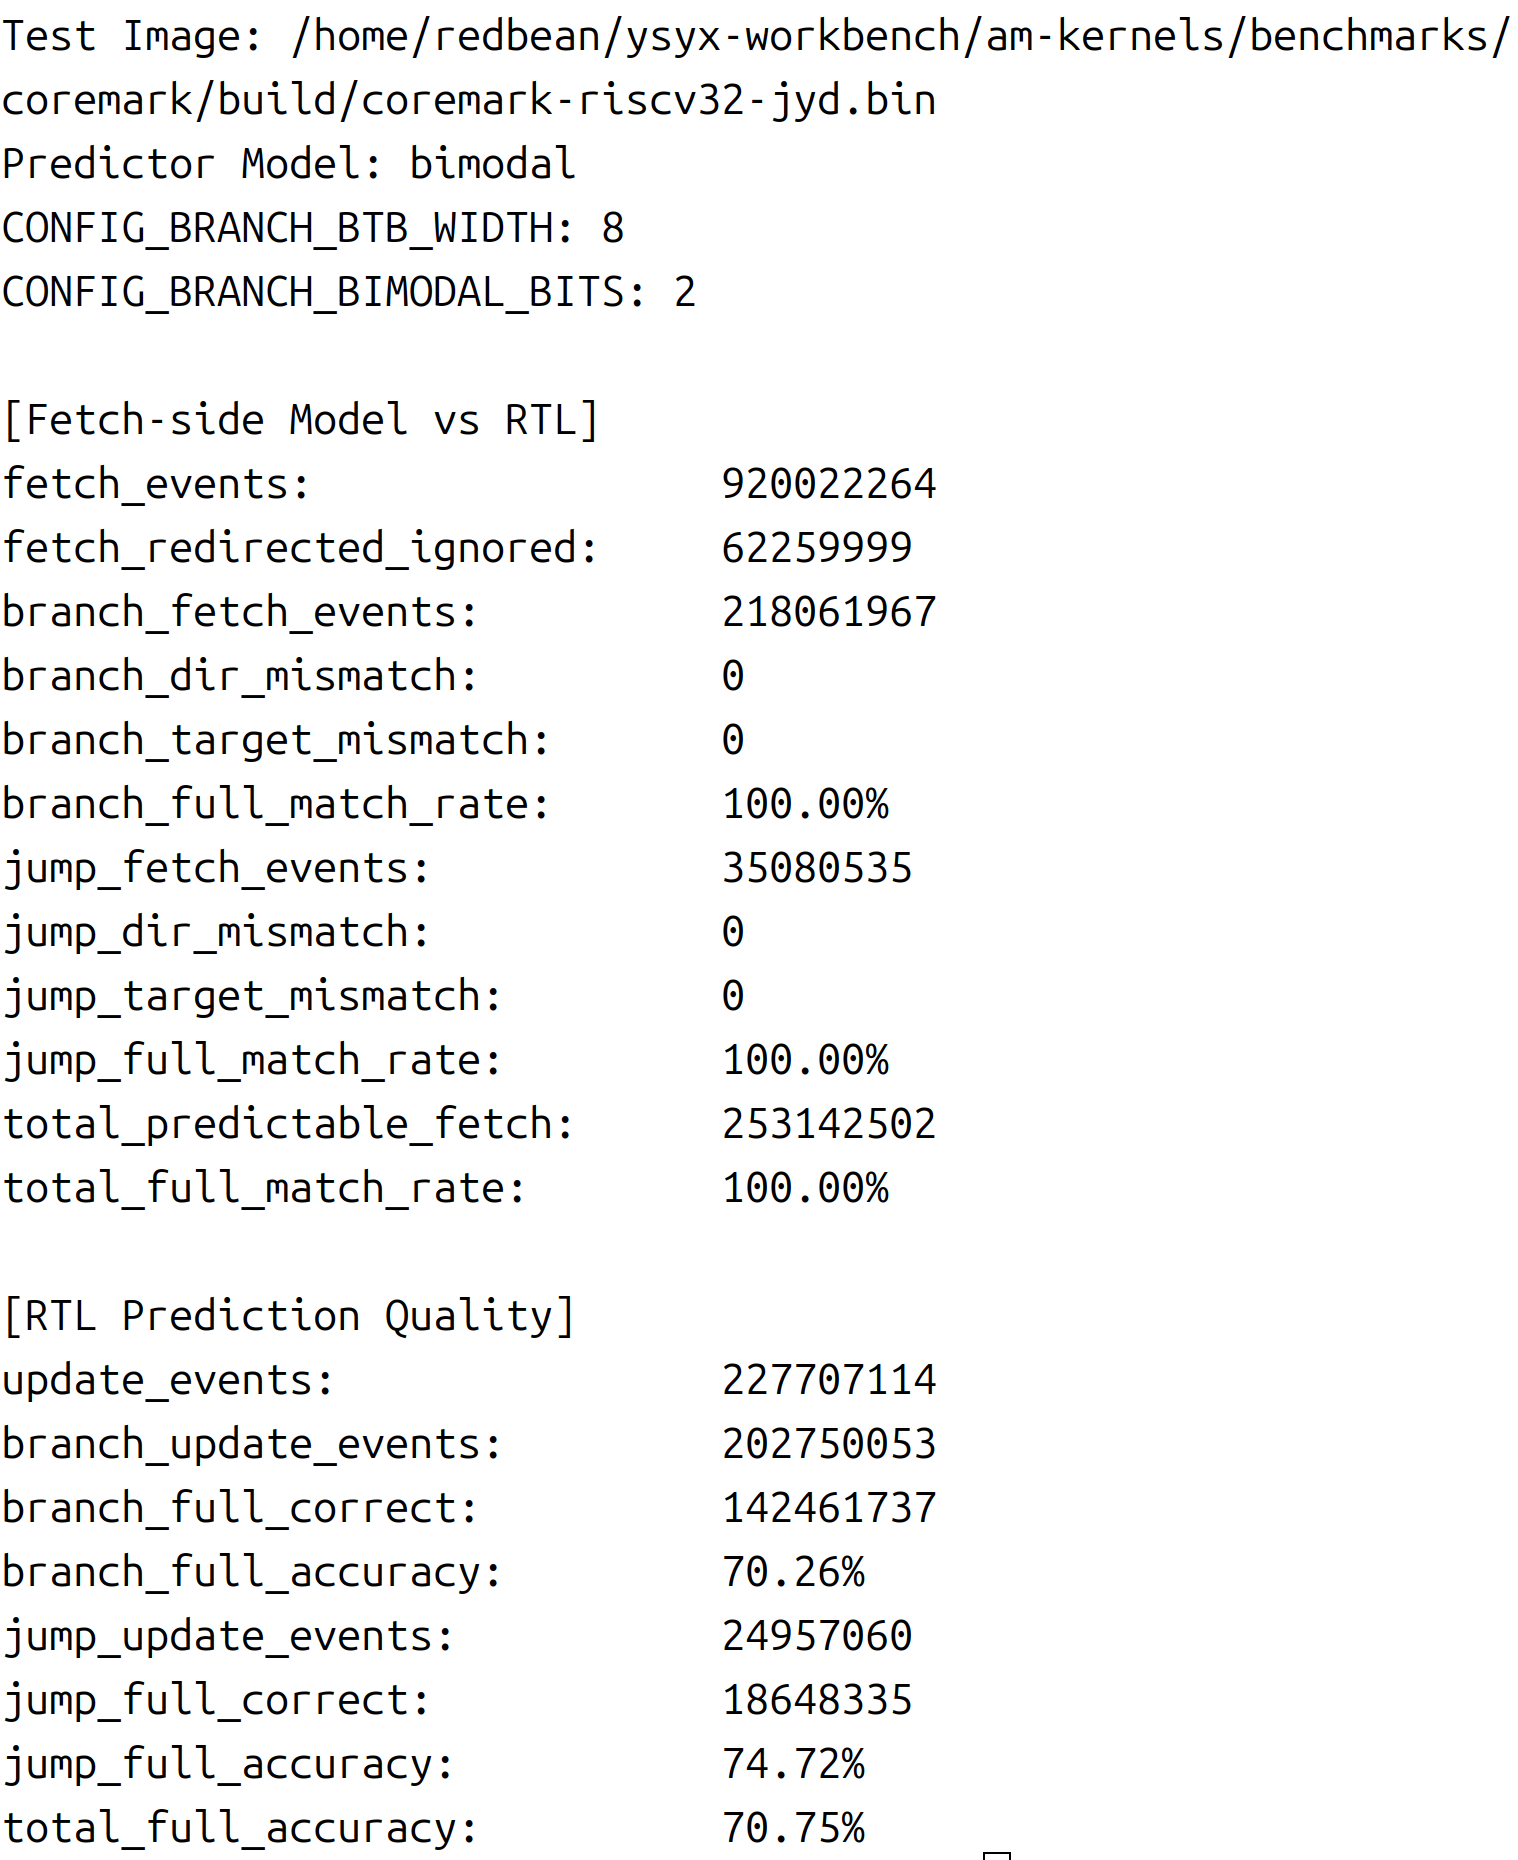
\includegraphics[width=0.90\linewidth]{figures/bimodal_sim.png}
  \caption{BPU测试结果（Bimodal）}
  \label{fig:bimodal_pass}
\end{figure}

\section{验证平台介绍}

\subsection{FPGA 平台型号}

验证平台为竞业达 FPGA 试验箱的数字孪生平台，芯片型号为 Xilinx Kintex-7。

\subsection{下载/烧录工具版本}

下载与烧录工具采用 2023.2 版本的 Vivado Hardware Manager。

\subsection{上电与串口交互测试说明}

上板验证时，首先完成工程综合、实现和比特流生成；随后登录数字孪生平台并从数据库加载对应开发板；最后通过 Vivado Hardware Manager 或数字孪生平台提供的烧录入口加载 bitstream。程序运行结果通过数字孪生平台界面的 LED、数码管和状态显示区域进行观察。

\section{SoC 集成}

基于官方提供的 SoC 模板集成设计的处理器核心，集成过程与修改内容如下：

修改地址映射以兼容官方 SoC；将存储数据的 DRAM 替换为更利于时序优化与布局布线的单端口 BRAM，同时对 DRAM 的驱动进行相应修改，以适配 BRAM 的读数据过程。

最终的 SoC 框架如图~\ref{fig:soc-framework} 所示。

\begin{figure}[H]
  \centering
  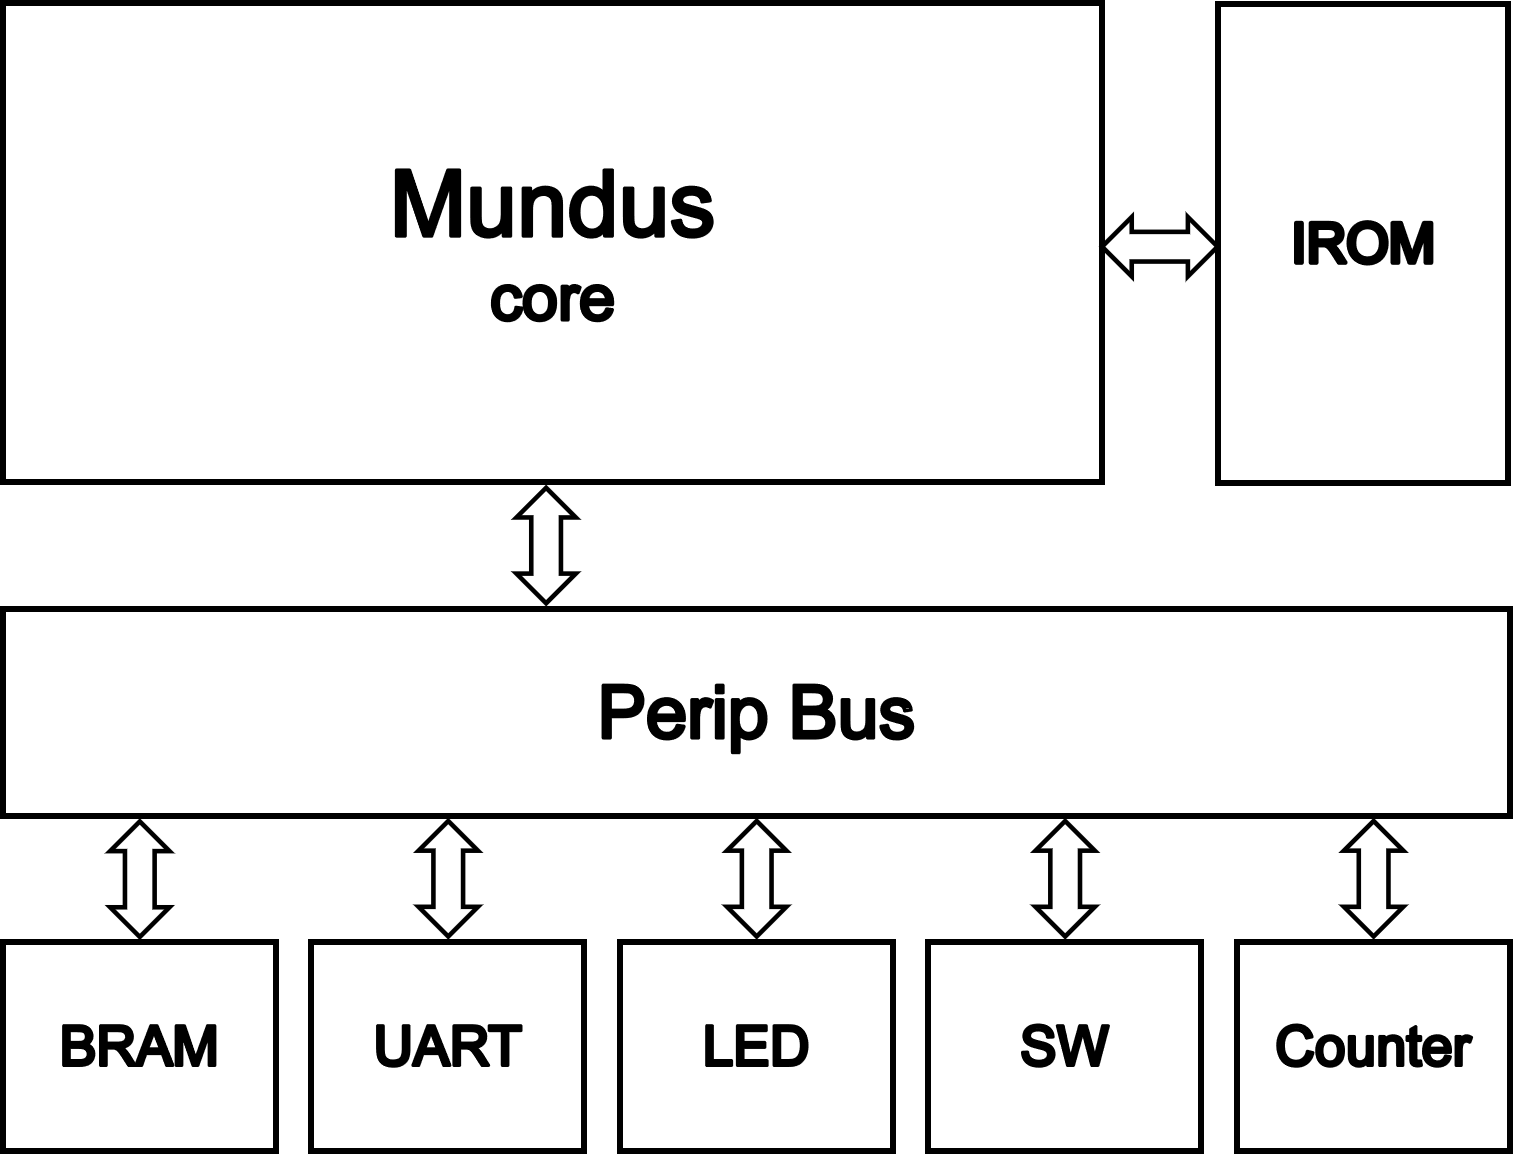
\includegraphics[width=0.70\linewidth]{figures/soc_framework.png}
  \caption{SoC 系统框架图}
  \label{fig:soc-framework}
\end{figure}

\section{测试用例说明}
\label{sec:test-cases}

\subsection{指令程序例程}
\label{subsec:instruction-test-programs}

官方提供了三个测评程序的 irom.coe 和 dram.coe，三个程序的 irom.coe 部分内容分别如图~\ref{fig:src0-coe}、图~\ref{fig:src1-coe} 和图~\ref{fig:src2-coe} 所示。

\begin{figure}[H]
  \centering
  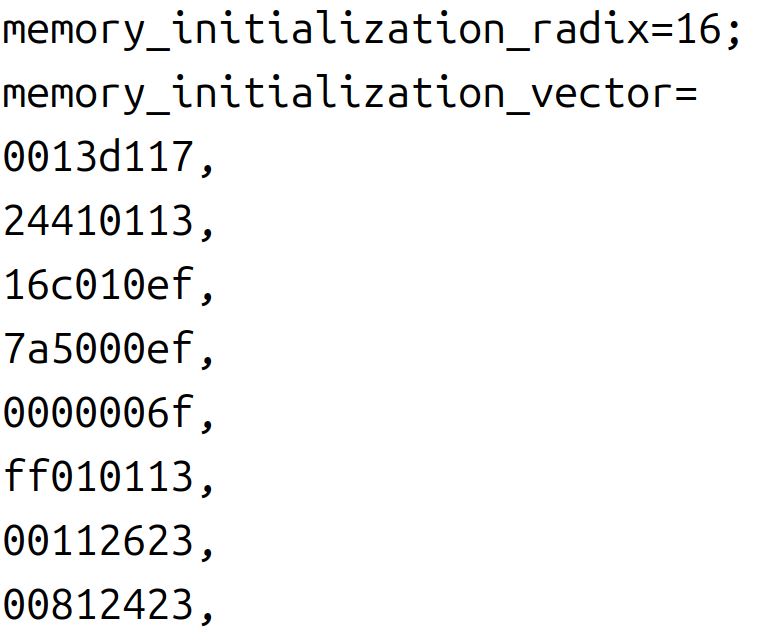
\includegraphics[width=0.70\linewidth]{figures/src0_irom_coe.png}
  \caption{src0 程序 irom.coe 部分内容}
  \label{fig:src0-coe}
\end{figure}

\begin{figure}[H]
  \centering
  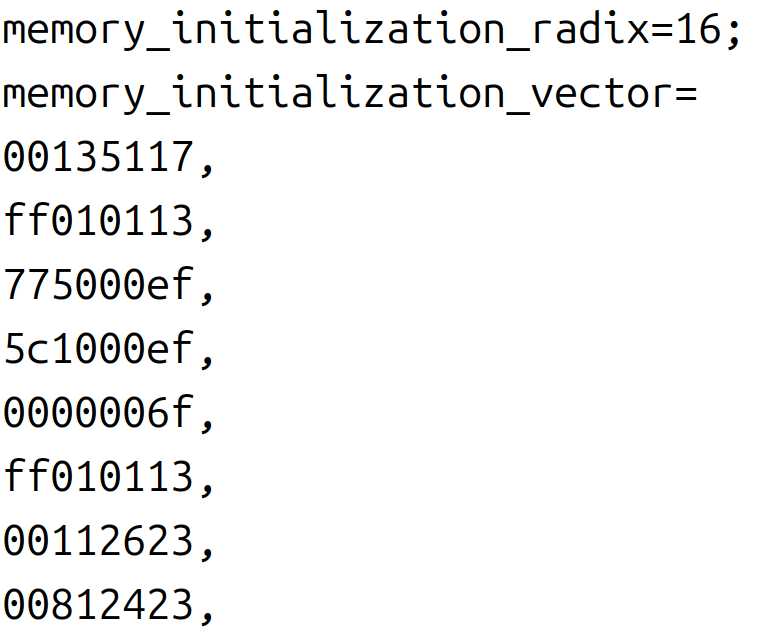
\includegraphics[width=0.70\linewidth]{figures/src1_irom_coe.png}
  \caption{src1 程序 irom.coe 部分内容}
  \label{fig:src1-coe}
\end{figure}

\begin{figure}[H]
  \centering
  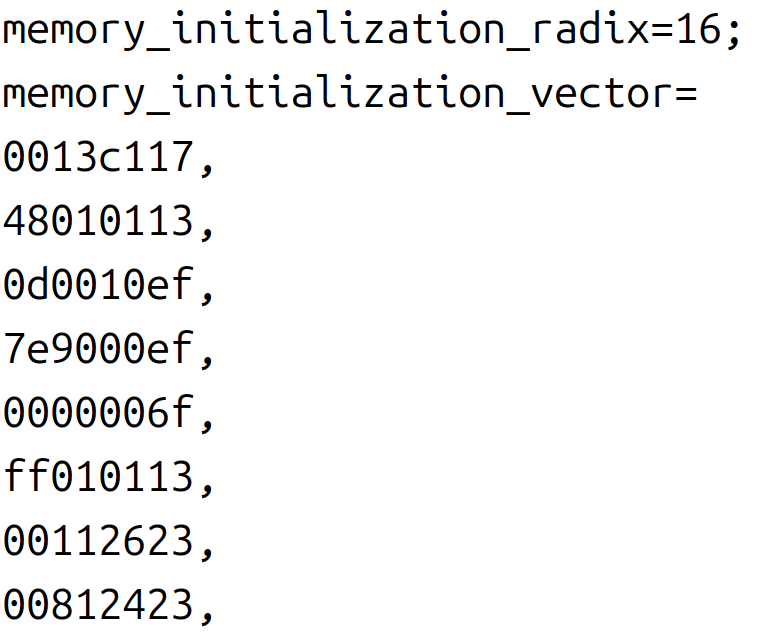
\includegraphics[width=0.70\linewidth]{figures/src2_irom_coe.png}
  \caption{src2 程序 irom.coe 部分内容}
  \label{fig:src2-coe}
\end{figure}

三个程序均可测试 RV32I 基础 37 条指令的实现情况与处理器性能，运行结果显示方式相同，具体说明如下。

若测试不通过，则可能出现多种情况：无法正常运行时，LED 及数码管无显示；能够正常运行但部分指令不通过时，左边两个数码管显示数据小于 37，且不进行性能测试；若指令测试均通过但性能测试不通过，则 LED 会显示叉号。

若测试成功，FPGA 开发板上的 LED 灯组应显示为勾号，左边两个数码管应显示通过测试的指令数量，右边六个数码管应显示程序测试所用时间，单位为毫秒。

\subsection{上板运行流程说明}

将官方模板中的处理器核心替换为队伍设计的处理器核心，生成比特流文件。为了提高处理器主频，综合与实现阶段配置了相应的策略及参数，分别如图~\ref{fig:synth-strategy} 和图~\ref{fig:impl-strategy} 所示。随后登录数字孪生平台，从数据库加载开发板，烧录比特流文件，最后在孪生平台界面显示程序运行结果。

\begin{figure}[H]
  \centering
  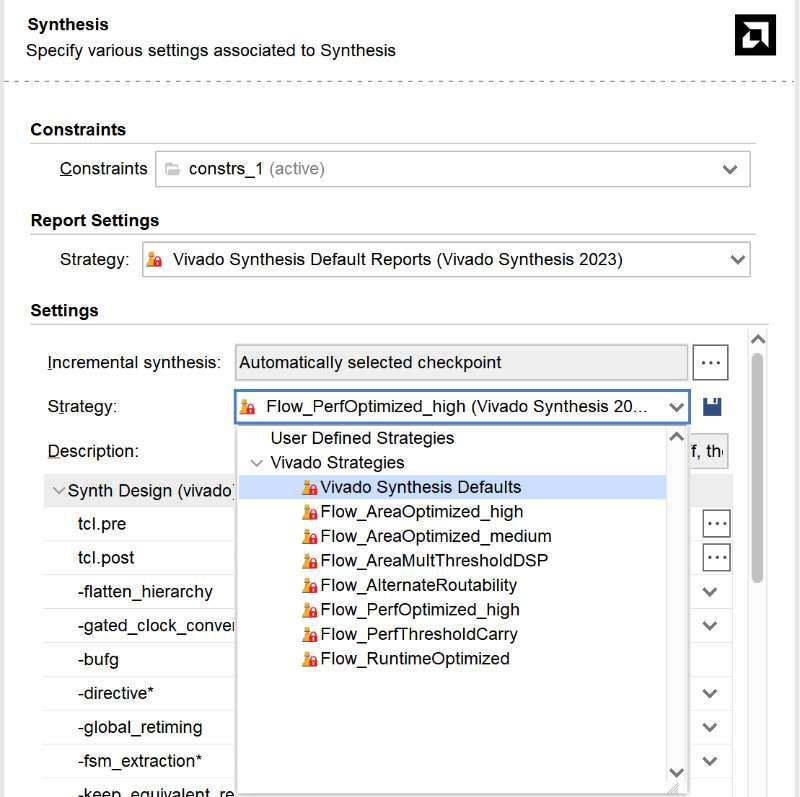
\includegraphics[width=0.82\linewidth]{figures/vivado_synthesis_strategy.jpg}
  \caption{综合策略及参数配置}
  \label{fig:synth-strategy}
\end{figure}

\begin{figure}[H]
  \centering
  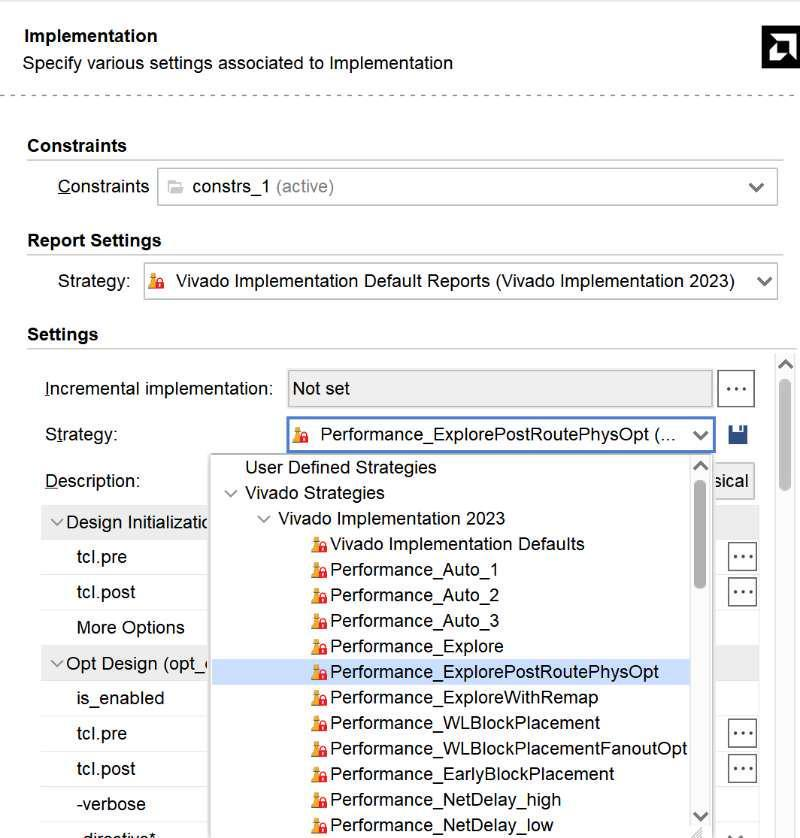
\includegraphics[width=0.82\linewidth]{figures/vivado_implementation_strategy.jpg}
  \caption{实现策略及参数配置}
  \label{fig:impl-strategy}
\end{figure}

\section{验证结果}

\subsection{数字孪生运行截图}

官方三个测试程序 src0、src1、src2 均通过，运行显示结果分别如图~\ref{fig:digital-src0}、图~\ref{fig:digital-src1} 和图~\ref{fig:digital-src2} 所示。

\begin{figure}[H]
  \centering
  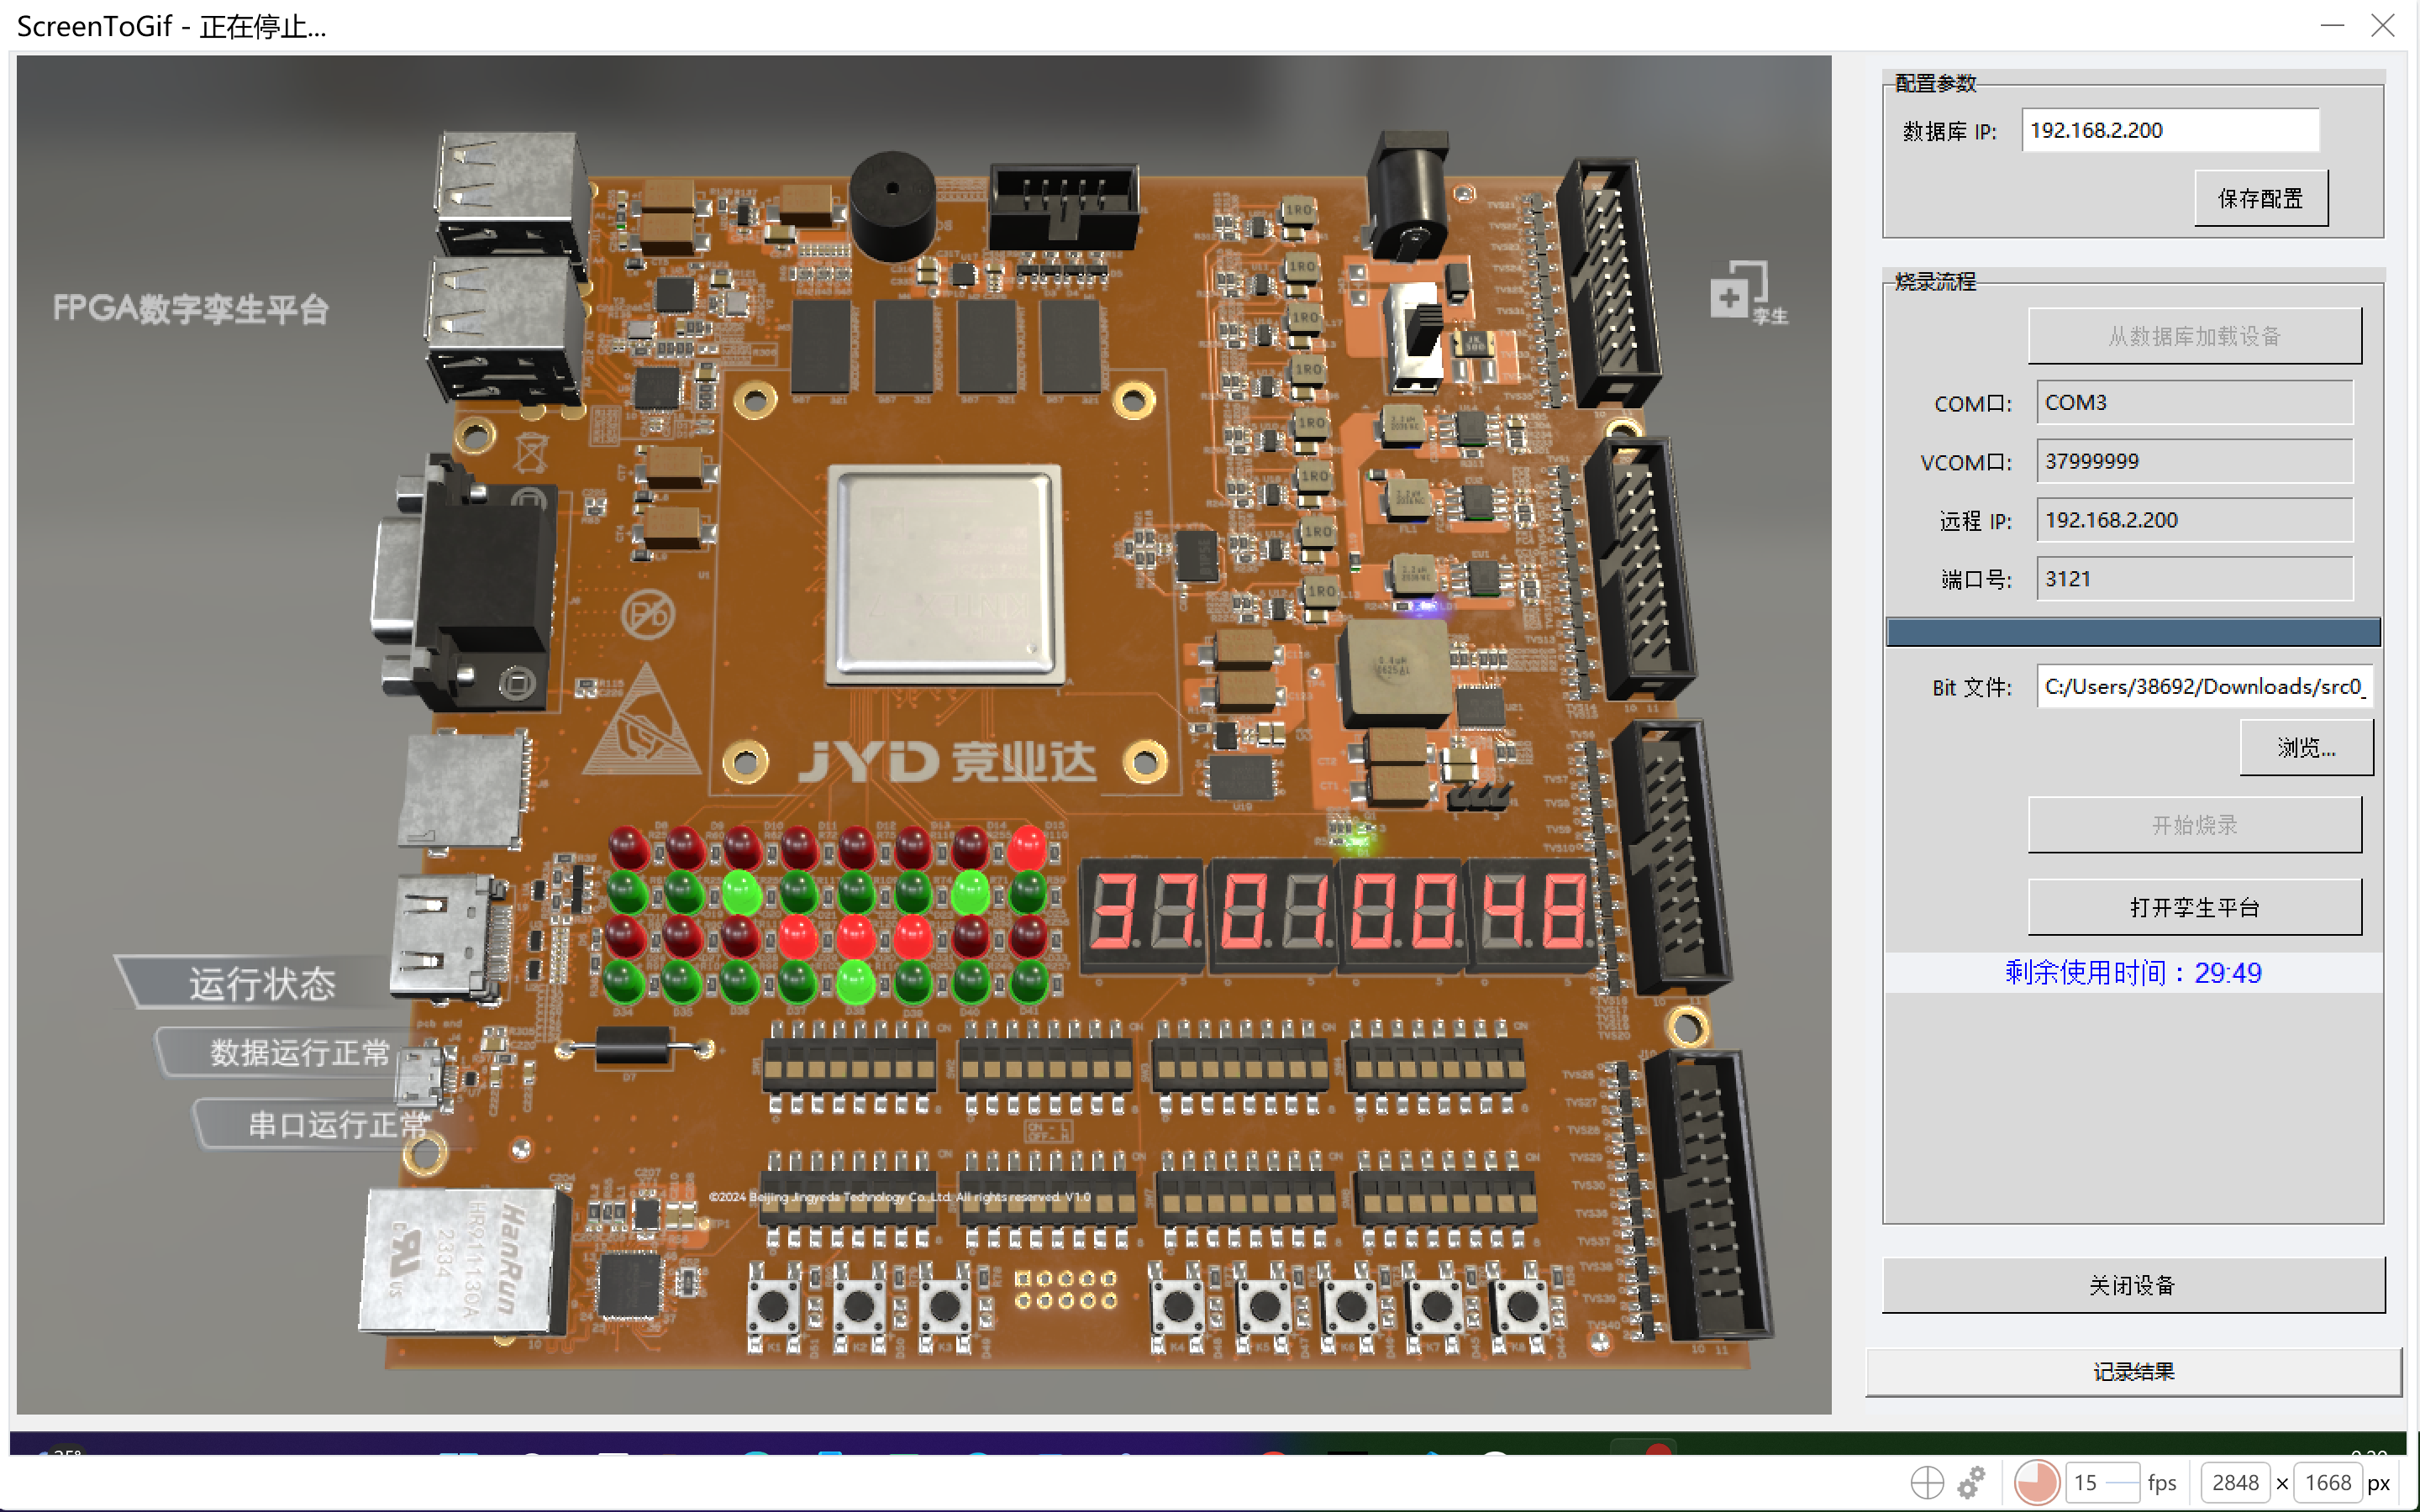
\includegraphics[width=0.95\linewidth]{figures/digital_twin_src0.png}
  \caption{src0 数字孪生运行结果}
  \label{fig:digital-src0}
\end{figure}

\begin{figure}[H]
  \centering
  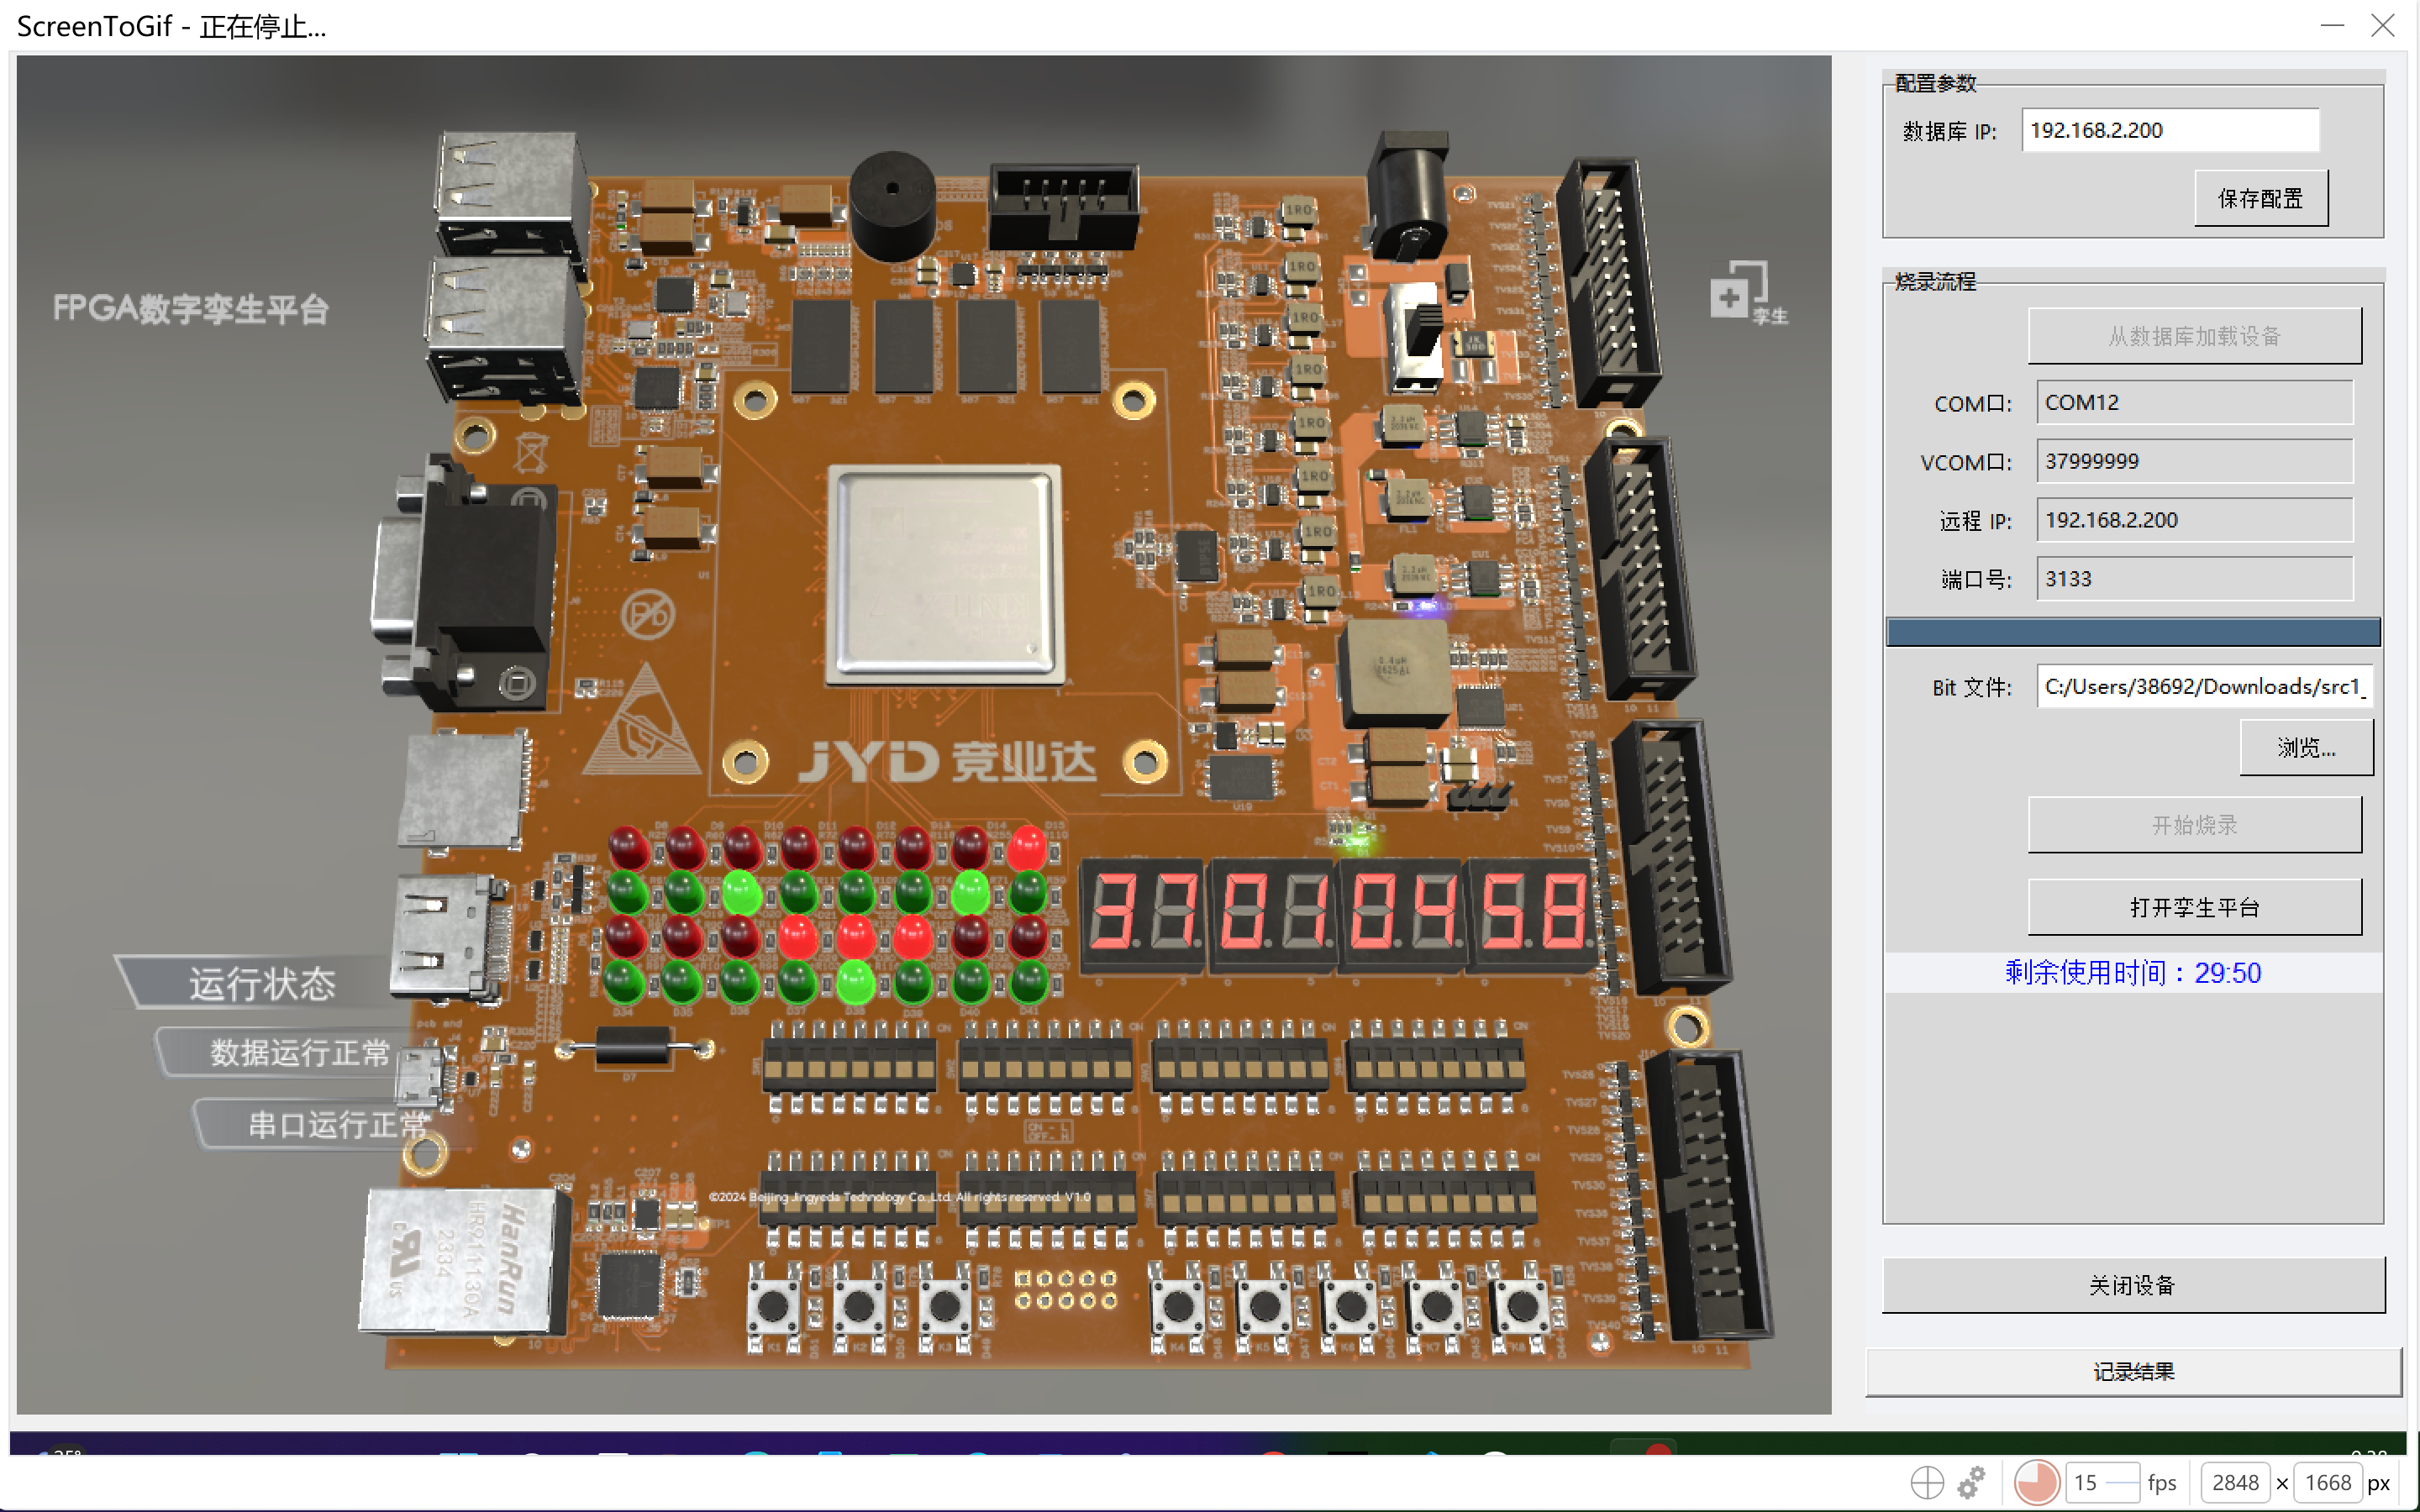
\includegraphics[width=0.95\linewidth]{figures/digital_twin_src1.png}
  \caption{src1 数字孪生运行结果}
  \label{fig:digital-src1}
\end{figure}

\begin{figure}[H]
  \centering
  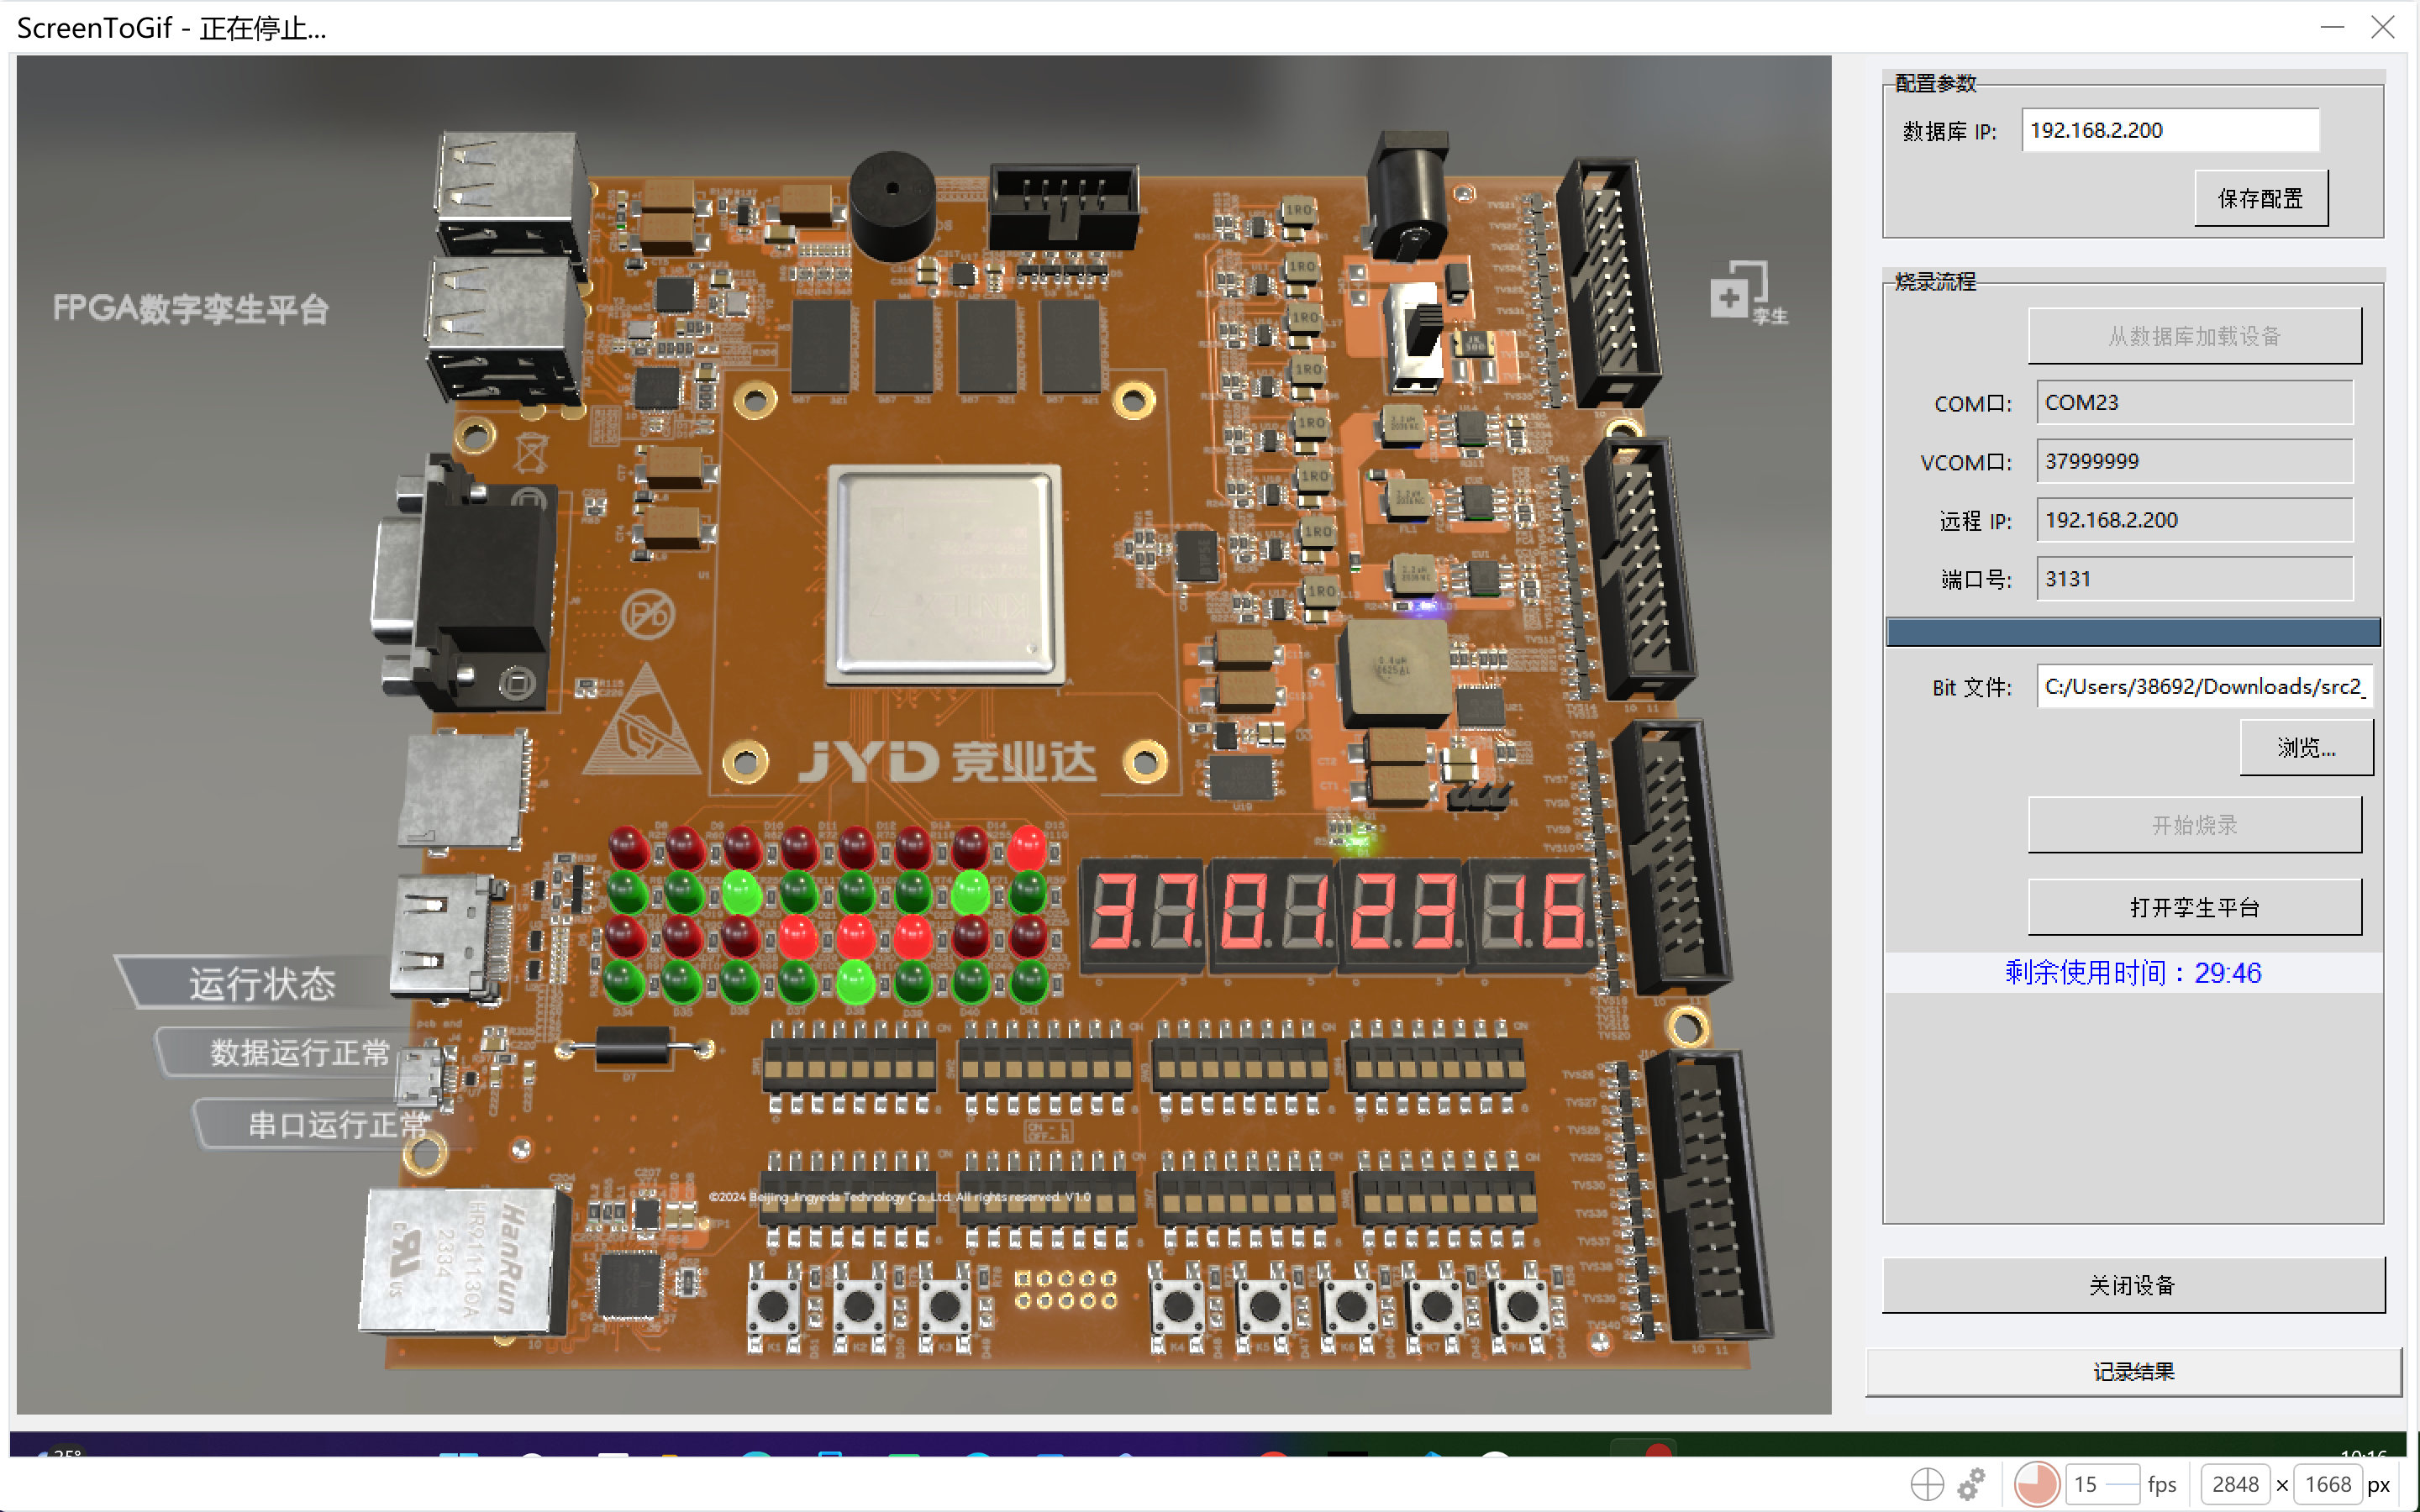
\includegraphics[width=0.95\linewidth]{figures/digital_twin_src2.png}
  \caption{src2 数字孪生运行结果}
  \label{fig:digital-src2}
\end{figure}

\subsection{验证结果总结说明}

板上验证结果与第~\ref{sec:test-cases} 节中的测试用例相对应。三个官方测试程序均能够在数字孪生平台上正常运行，LED 显示为通过状态，数码管显示通过 37 条 RV32I 基础指令测试，并给出对应程序运行耗时。该结果说明处理器核心在集成至官方 SoC 后，能够正确完成指令功能测试和基础性能测试。

\subsubsection{功能与性能结果分析}

集成于官方 SoC 上的六级流水处理器在上板测试中最终可超频达到 200 MHz。结合表~\ref{tab:digital-twin-result} 可知，三个官方测试程序均通过 RV32I 的 37 条基础指令测试，说明处理器在数字孪生平台上具备稳定的功能正确性和较好的综合运行性能。

\begin{table}[H]
  \centering
  \caption{官方测试程序数字孪生运行结果}
  \label{tab:digital-twin-result}
  \begin{normaltable}
  \resizebox{0.70\linewidth}{!}{%
  \begin{tabular}{@{}ccccc@{}}
    \toprule
    测试程序 & 运行频率 & 指令测试通过数 & 显示运行时间 & 结果 \\
    \midrule
    src0 & 200 MHz & 37 & 10048 ms & 通过 \\
    src1 & 200 MHz & 37 & 10458 ms & 通过 \\
    src2 & 200 MHz & 37 & 12316 ms & 通过 \\
    \bottomrule
  \end{tabular}
  }
  \end{normaltable}
\end{table}

\subsubsection{资源使用及面积、功耗分析}

根据资源和面积报告可知，由于使用了 BRAM 代替了 DRAM，节省了大量的 LUTRAM 使用和面积占用，故目前的处理器设计使用的资源较少，LUT、LUTRAM、FF 仅分别使用了 2\%、1\% 和 1\%，仍有充足余裕可供进一步开发。

\begin{figure}[H]
  \centering
  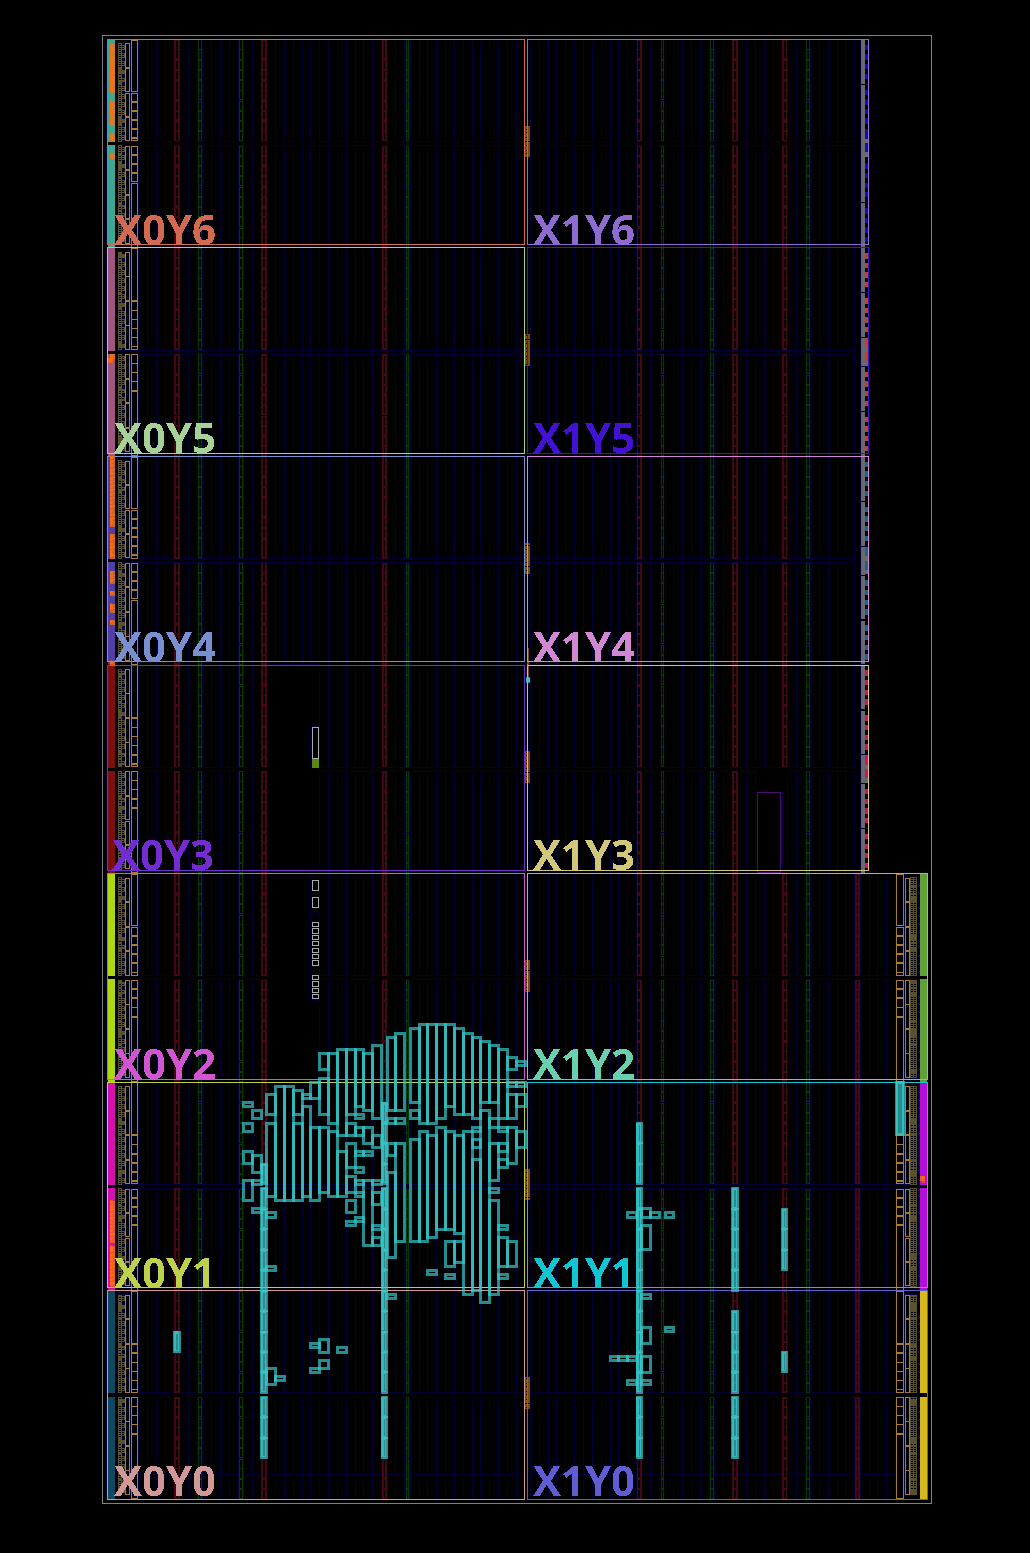
\includegraphics[width=0.82\linewidth]{figures/area_analysis.jpeg}
  \caption{综合面积}
  \label{fig:area-placeholder}
\end{figure}

\begin{figure}[H]
  \centering
  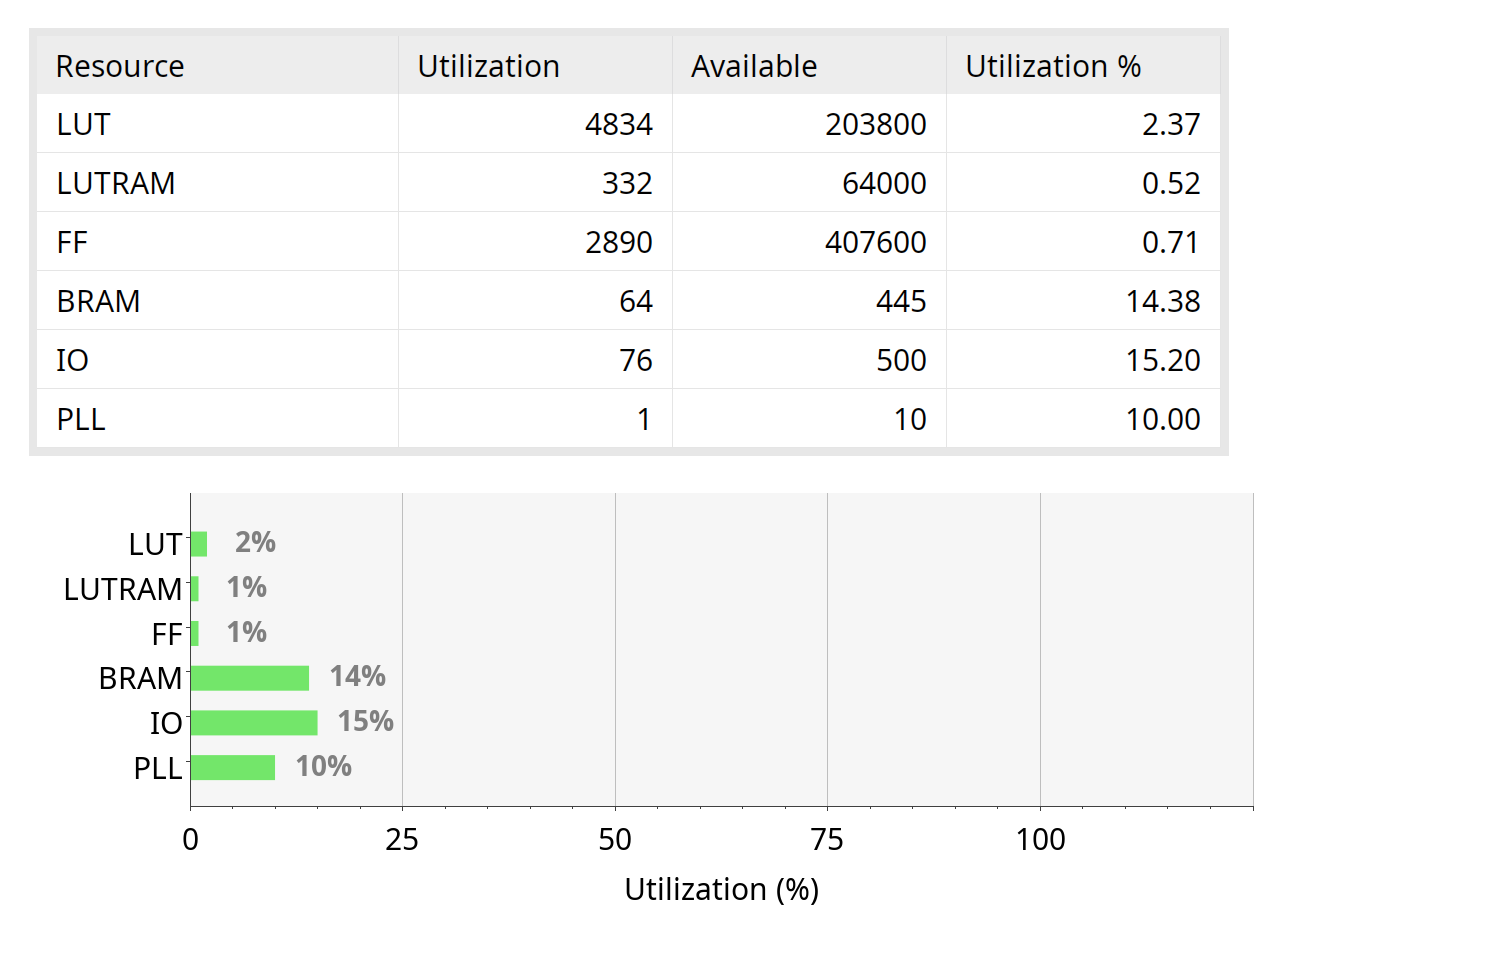
\includegraphics[width=0.82\linewidth]{figures/resource_usage.jpeg}
  \caption{资源使用}
  \label{fig:resource-placeholder}
\end{figure}

由功耗报告可知，芯片总功耗为 0.167W，动态功耗占比为总功耗的 70\%，静态功耗占比为总功耗的 30\%。而在动态功耗中，Clock、Signals、以及 Logic 的
占比各自为 11\%、34\%和 20\%。具体数据如图~\ref{fig:power-placeholder} 所示。

\begin{figure}[H]
  \centering
  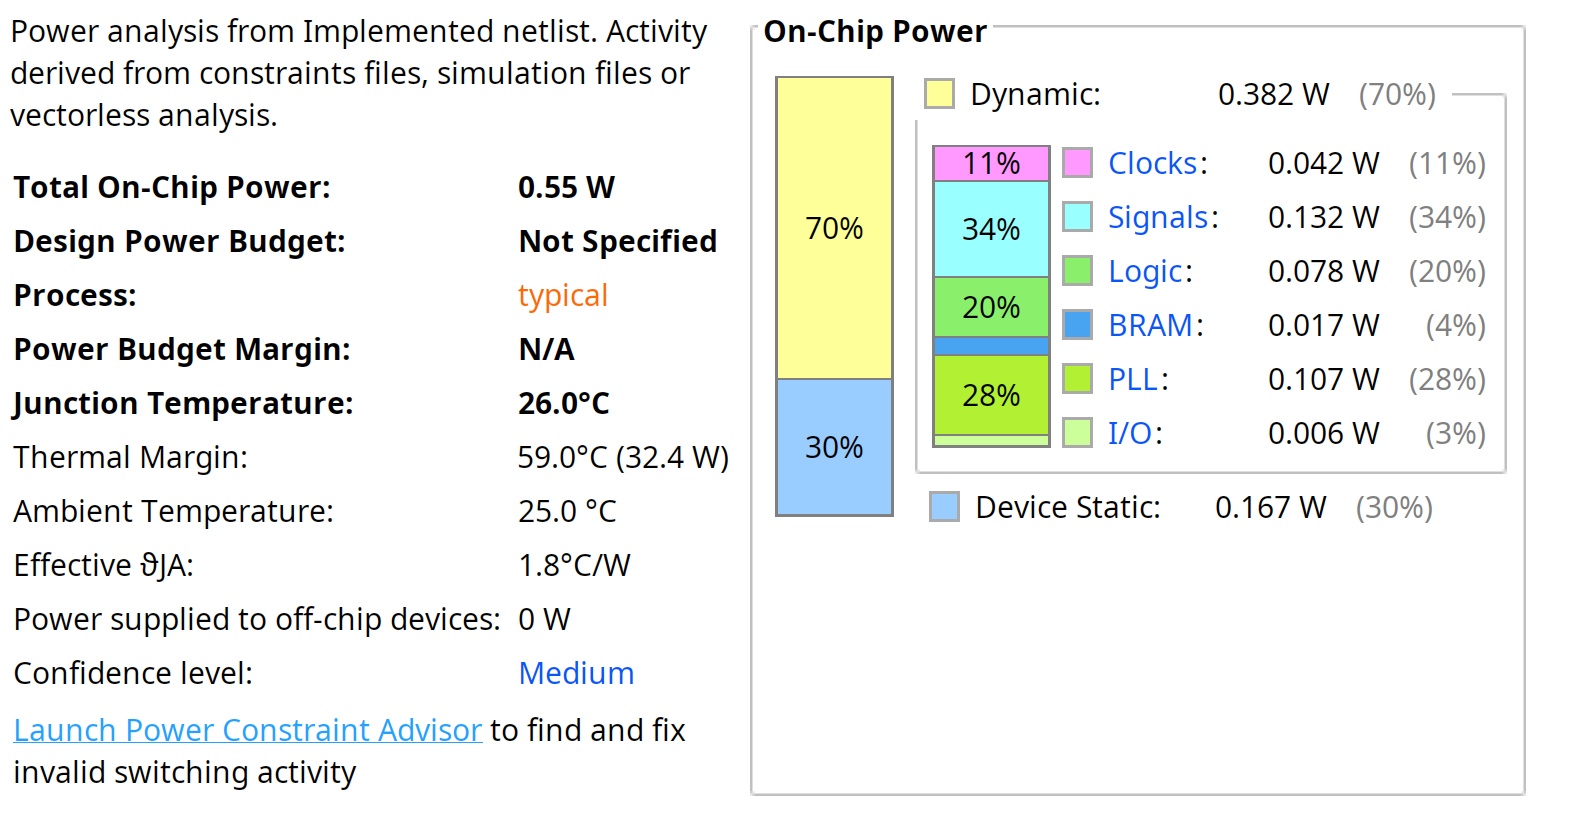
\includegraphics[width=0.82\linewidth]{figures/power_analysis.jpeg}
  \caption{功耗占比}
  \label{fig:power-placeholder}
\end{figure}

\end{document}
